\chapter{Biophysical background}\label{chap:biophys-back}

%\section{Basics of protein structure and their functionality}\label{sec:protein-struct-fun}
%Proteins, being at the center of action in biological processes, are one of the essential components of living systems. Nearly all the molecular transformations that define cellular metabolism are mediated by protein catalysts. Proteins also perform regulatory roles, monitoring extracellular and intracellular conditions and relaying information to other cellular components. In addition, they are essential structural components of cells.
% and serve as transporters that carry specific substances into or out of cells. 
%A complete list of known protein functions would contain many thousands of entries, including proteins that transport other molecules and proteins that generate mechanical and electrochemical forces, and such a list would not account for the thousands of proteins whose functions are not yet fully characterized or, in many cases, are completely unknown. 
%\cite{voet2016fundamentals}\\
%\\
%Proteins, long polymers of amino acids, constitute the largest fraction (besides water) of a cell. Some proteins have catalytic activity and function as enzymes; others serve as structural elements, signal receptors, or transporters that carry specific substances into or out of cells. 
%Proteins are perhaps the most versatile of all biomolecules; a catalog of their many functions would be very long. The sum of all the proteins functioning in a given cell is the cell's proteome, and proteomics is the systematic characterization of this protein complement under a specific set of conditions.
%Proteins, polynucleotides, and polysaccharides have large numbers of monomeric subunits and thus high molecular weights--in the range of 5,000 to more than 1 million for proteins, up to several billion for nucleic acids, and in the millions for polysaccharides such as starch. Individual lipid molecules are much smaller (Mr 750 to 1,500) and are not classified as macromolecules, but they can associate noncovalently into very large structures. Cellular membranes are built of enormous noncovalent aggregates of lipid and protein molecules. 
%All proteins, whether from the most ancient lines of bacteria or from the most complex forms of life, are constructed from the same ubiquitous set of 20 amino acids, covalently linked in characteristic linear sequences. Because each of these amino acids has a side chain with distinctive chemical properties, this group of 20 precursor molecules may be regarded as the alphabet in which the language of protein structure is written. What is most remarkable is that cells can produce proteins with strikingly different properties and activities by joining the same 20 amino acids in many different combinations and sequences. From these building blocks different organisms can make such widely diverse products as enzymes, hormones, antibodies, transporters, muscle fibers, the lens protein of the eye, feathers, spider webs, rhinoceros horn, milk proteins, antibiotics, mushroom poisons, and myriad other substances having distinct biological activities
%\cite{nelson2008lehninger}\\

Proteins are one of the essential components of living systems. Along with nucleic acids, proteins constitute the macromolecules that play a fundamental role in biology. 
Nucleic acids, in the form of DNA (DeoxyriboNucleic Acid) and RNA (RiboNucleic Acid), store and distribute the genetic information as needed, while proteins, contributing to the structure of an organism and executing most of the tasks required for it to function, are at the center of action in the majority of the biological processes.
%Proteins contribute to the structure of an organism and execute most of the tasks required for it to function. 
%Proteins even form part of the complex mechanism by which they are synthesized. Polysaccharides, linear and branched-chain polymers of sugars, provide structural elements, store energy, and when combined with peptides or proteins, play an important role in antigenicity and, more generally, in cellular recognition. Lipids, which include molecules such as fatty acids, phospholipids, and cholesterol, serve as energy sources and are the most important components of the membrane structures that organize and compartmentalize cellular function. 
 
Nearly all the molecular transformations that define cellular metabolism are mediated by protein catalysts. Proteins also perform regulatory roles, monitoring extracellular and intracellular conditions and relaying information to other cellular components. In addition, they are essential structural components of cells.
% and serve as transporters that carry specific substances into or out of cells. 
A complete list of known protein functions would contain many thousands of entries, including proteins that transport other molecules and proteins that generate mechanical and electrochemical forces, and such a list would not account for the thousands of proteins whose functions are not yet fully characterized or, in many cases, are completely unknown
\cite{voet2016fundamentals}.

%Proteins contribute to the structure of an organism and execute most of the tasks required for it to function. Proteins even form part of the complex mechanism by which they are synthesized. 
%Polysaccharides, linear and branched-chain polymers of sugars, provide structural elements, store energy, and when combined with peptides or proteins, play an important role in antigenicity and, more generally, in cellular recognition. Lipids, which include molecules such as fatty acids, phospholipids, and cholesterol, serve as energy sources and are the most important components of the membrane structures that organize and compartmentalize cellular function.
%In this volume we concentrate on globular proteins, the biological macro- molecules with the greatest functional range. 
%It is for these systems that the relation of function to structure and dynamics is best understood. 
In particular, most chemical transformations that occur in living systems are catalyzed by enzymes, the globular proteins that have evolved for executing such specific tasks. 
As well as enhancing the rates of reactions, sometimes by eight or more orders of magnitude, globular proteins inhibit certain reactions (for instance, the transcription of DNA) involved in the mechanism for the control of growth and differentiation. A breakdown of these control mechanisms can lead to unobstructed growth and the development of cancer. 
Other proteins (such as hemoglobin) serve to transport small molecules (such as oxygen), electrons, and energy to the appropriate parts of the organism. 
Antibody molecules are proteins that protect the organism by specifically recognizing and binding to foreign antigenic substances (such as viruses). 
Many proteins have structural roles; for example, fibrous tissue is composed mainly of the protein collagen, and the major functional components of muscles are proteins
\cite{brooks1988proteins}.

Because of this wide range of protein functions and the need to develop specialized proteins for each of them, the number of different proteins in an organism can be very large and, in particular, they constitute the largest fraction (besides water) of a cell. The well-studied bacterium \textit{Escherichia coli}\footnote{Commonly abbreviated E. coli, Escherichia coli is a bacterium frequently used as a model organism in microbiology studies, thanks to its long history of laboratory culture and ease of manipulation.} contains about 3000 different kinds of proteins. Since many of them occur in multiple copies, there are a total of about 1 million protein molecules in a single bacterium. In human beings it is estimated that there are more than $10^5$ different proteins.

For most proteins, the biological function includes an interaction with one or more small molecules or with another macromolecule. 
Whether reactive or nonreactive systems are being considered, there can be important conformational alterations in the protein and related changes can also occur in the bounded molecule structure. Such concerted conformational changes are the essential element for activity in some cases; in others, they play a less significant role.
In hormone-receptor binding, for example, the structural changes induced in the receptors are fundamental to the transmission of information. 
Correspondingly, the conformational transition induced by ligand binding in hemoglobin is an integral part of the cooperative mechanism.
Further, in many systems, small motions have been observed (e.g., the differences between the ligated and unligated structure of ribonuclease A) that appear to be involved in the function of the protein. 
Thus any attempt to understand the details of the activity of proteins requires an investigation of the dynamics of the structural fluctuations and their relation to reactivity and conformational change
\cite{brooks1988proteins}.

%In addition to their biological importance, proteins are intrinsically interesting systems from the viewpoint of physical chemistry. They are long-chain polymers, but unlike most polymers they have a well-defined average structure. This structure is aperiodic in the sense that it does not have regular repeats. Since the structure is determined by weak, noncovalent, interactions among the elements of the polypeptide chain, large fluctuations are expected. For a complete description of proteins, it is important, therefore, to know, in addition to the average structure, the form of the fluctuations that occur, to determine how they take place, and to evaluate their magnitudes and time scales.

%Although to chemists and physicists it is self-evident that polymers such as proteins undergo significant fluctuations at room temperature, the classic view of such molecules in their native state had been static in character. This followed from the dominant role of high-resolution X-ray crystallography in providing structural information for these complex systems. The remarkable detail evident in crystal structures led to an image of biomolecules with every atom fixed in place. Tanford suggested that as a result of packing considerations ``the structure of proteins must be quite rigid.'' D. C. Phillips, who determined the first enzyme crystal structure, has written: ``The period 1965-75 may be described as the decade of the rigid macromolecule. Brass models of DNA and a variety of proteins dominated the scene and much of the thinking.'' Molecular dynamics simulations have been instrumental in changing the static view of the structure of biomolecules to a dynamic picture. It is now recognized that the atoms of which biopolymers are composed are in a state of constant motion at ordinary temperatures. The X-ray structure of a protein providesthe average atomic positions, but the atoms exhibit fluidlike motions of sizable amplitudes about these averages. Crystallographers have acceded to this viewpoint and have come so far as sometimes to emphasize the parts of a molecule they do not see in a crystal structure as evidence of motion or disorder. The new understanding of protein dynamics subsumes the static picture. Knowledge of the average atomic positions allows discussion of many aspects of biomolecule function in the language of structural chemistry. However, recognition of the importance of fluctuations opens the way for more sophisticated and accurate interpretations of protein activity.

%Simulations of proteins, as of many other systems (e.g., liquids), can, in principle, provide the ultimate details of motional phenomena. The primary limitation of simulation methods is that they are approximate. It is here that experiment plays an essential role in validating the simulation methods; that is, comparisons with experimental data serve to test the accuracy of the calculated results and provide criteria for improving the methodology. However, the experimental approaches to biomolecular dynamics are limited as to the information that can be obtained from them; e.g., if one is concerned with the time scale of motions, the frequency spectrum covered by experiments such as nuclear magnetic resonance (NMR) is incomplete, so that motional models that are able to rationalize the data can be inaccurate. When experimental comparisons indicate that the simulations are meaningful, their capacity for providing detailed results often makes it possible to examine specific aspects of the atomic motions far more easily than by making measurements. How- ever, at the present stage of development, possible inaccuracies in the simulations must be kept in mind in evaluating and applying the results
%\cite{brooks1988proteins}.


\section{Macromolecules in biology: the polymeric nature of proteins}\label{sec:polym-prot}
Proteins, as well the nucleic acids, are among the most important molecules in biology. 
Generally, molecules are generated by the formation of covalent bonds between pairs of atoms, in which the two atoms share electrons. A covalent bond forms when atoms individually do not have enough electrons for a complete octet: if two atoms can complete their octets by sharing electrons, they can do so by forming a covalent bond. Covalent bonds can be explained only by quantum mechanics, however, due to the high complexity of biological systems that involve many atoms of different types, a quantum mechanical treatment of these systems is not feasible.
The general way to solve this problem is to use a semiclassical approach based on empirical approximations derived from experimental results and quantum mechanical simulations of small compounds. In particular, the main concept that is very useful to consider is that covalent bonds are generally not broken in isolation under most conditions experienced in molecular biology\footnote{This is true because, in biological environments, the thermal energy of a system is often more than two orders of magnitude smaller than the typical covalent binding energy: $k_B T \approx 4 \cdot 10^{-21} J \; << \; E_{\text{binding}} \approx (3 \div 10) \cdot 10^{-19} J$. Hence, the probability that, as a consequence of the thermal agitation, the covalent bond between two isolated atoms spontaneously breaks is usually negligible.}. When a covalent bond is broken, as in a chemical or enzymatic reaction, it is generally exchanged with another covalent bond to a different atom. Consequently, covalent bonds define the structures and properties of small molecules, and those of large molecules are determined by the covalent structures of the smaller substituents from which they are made.

Proteins and nucleic acids are macromolecules characterized by their very large sizes and high molecular weights. These giant molecules can contain many thousands, millions, even billions, of atoms. Fortunately, they are polymers, i.e. long molecular chains built up by the repetition of a few relatively simple subunits, the monomers, that are linked together in a linear fashion. The polymeric nature of these biomolecules, in spite of their huge dimension, lead to a simplification of their description -- the basic properties of a polymer are determined by those of simpler molecules (its constituent monomers) and by the arrangement of these monomers within the polymeric chain. In particular, the monomers that occur in a polymeric chain can be one of four distinct nucleotides, for nucleic acids, while they can be one of 20 different amino acids in the case of proteins. It is interesting to note that the number of distinct monomers from which proteins are made is considerably greater than that of nucleic acids and, in addiction, they have widely differing chemical and physical properties. As a consequence, this leads proteins to lack a distinctive uniform and regular structure such for the nucleic acids (tipically double helix for DNA, whereas single helix for RNA). Instead, different proteins can have totally different well-defined average structures \cite{voet2016fundamentals}.
%The 20 kinds of amino acids from which proteins are made have widely differing chemical and physical properties. This lead proteins to do not have uniform, regular structures such for case of the nucleic acids (tipically double helix for DNA, whereas single helix for RNA). Instead, different proteins have different well-defined average structures \cite{voet2016fundamentals}.

Anyway, both for proteins and nucleic acids, each monomer of the polymeric chain consists of two parts: 
the group of atoms X, common to all monomers, that  is the constant repeating part of the polymer and the side chain R$_i$ that, being  the remaining atoms of the monomer, represents the variable part of the chain and is specific to each amino acid (indeed the side chain R$_i$ identifies the type of $i$-th monomer among the several possible: 4 for nucleic acids -- 20 for proteins).

\begin{figure}[h]
\centering
\begin{minipage}[t]{0.75\textwidth}
\centering
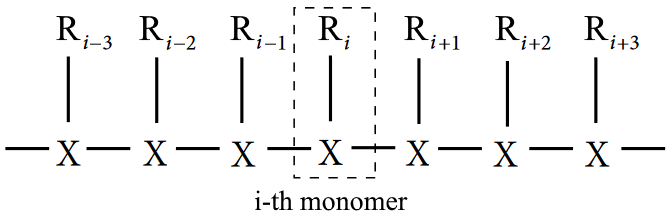
\includegraphics[width=0.7\textwidth]{Polymer-v3.png}

\caption{\small{Simple schematization of a section of an organic polymer such as DNA, RNA or proteins. An X represents the group of those atoms of a monomer that, with the other X groups of the other monomers, build up the backbone. R$_i$ represent the side chain specific of the $i$-th monomers.
    \textit{Source:} T. E. Creighton, ``\textit{The Biophysical Chemistry of Nucleic Acids \& Proteins}'' (2010) 
    \cite{creighton2010biophysical}.}
}


\label{fig:Polymer}
\end{minipage} 
\end{figure}

The backbone of a polymer is the longest series of covalently bonded atoms that create the continuous chain of the macromolecule (in figure \ref{fig:Polymer}, the backbone is identified by the sequence of the X groups)\footnote{Polymers are subdivided into organic, which have a carbon backbone, and inorganic which have backbones containing only main group elements.}. %The side-chains are the chemical groups of each monomer that are attached to the core part of the respective molecules that form the backbone.

In homopolymers, the side-chains connected to the backbone are all the same, as in carbohydrates or polymers made chemically, while in copolymers they are variable; the natural proteins and nucleic acids are extreme examples with several different types. In any case, the backbone has primarily a structural role, while the side-chains contain the functional groups. In spite of the enormous sizes of proteins and nucleic acids, it is possible to determine their detailed covalent structures because, knowing the detailed structures of all the possible monomers, it is only necessary to determine their linear sequence in the polymer.

Hence, the detailed structures of the monomers are extremely important, because they determine the global properties of the macromolecule. They occur many times in the polymer, and their structures are multiplied many times over. While these details of the structure might seem very minor and negligible, they have extremely important consequences for the three-dimensional (3-D) structures of biopolymers and their functions. These consequences even extend to the macroscopic level; for example, the left/right asymmetry of all but the simplest microorganisms is believed to result from asymmetry at the atomic level of certain molecules
\cite{creighton2010biophysical}. In the next section a brief summary of the structures and chemical properties of the common amino acids is presented. 

\section{The building blocks of proteins: amino acids}\label{sec:amino-acids}

Proteins can be broken down (hydrolyzed) to their constituent amino acids by a variety of methods, and the earliest studies of proteins naturally focused on the free amino acids derived from them. Twenty different amino acids are commonly found in proteins. The first to be discovered was asparagine, back in 1806. 
In spite of the great number of amino acids discovered in nature during the years (more then 700), the analyses of a vast number of proteins from almost every conceivable source have shown that all proteins are composed of 20 standard amino acids
\cite{wu2013amino}. 
The last of the 20 to be found, threonine, was not identified until 1938. All the amino acids have trivial or common names, in some cases derived from the source from which they were first isolated. Asparagine was first found in asparagus, and glutamate in wheat gluten; tyrosine was first isolated from cheese (its name is derived from the Greek tyros,``cheese''); and glycine (Greek glykos, ``sweet'') was so named because of its sweet taste.
\cite{nelson2008lehninger}

%Amino acids are organic compounds containing amine (-NH2) and carboxyl (-COOH) functional groups, along with a side chain (R group) specific to each amino acid. The key elements of an amino acid are carbon (C), hydrogen (H), oxygen (O), and nitrogen (N), although other elements are found in the side chains of certain amino acids. In spite of the great number of amino acids discovered in nature (more then 700), the analyses of a vast number of proteins from almost every conceivable source have shown that all proteins are composed of 20 standard amino acids
%\cite{wu2013amino}. 
The 20 common amino acids have the same basic structure which is shown in Fig. \ref{fig:AminoAcid}. %Amino acids that have an amino group bonded directly to the alpha-carbon are referred to as alpha amino acids
They have a carboxyl group --COOH (namely, a C atom double bonded to one O atom and singly bonded to another O atom that, in turn, is bonded with an H atom), an amino group --NH$_2$ (i.e. a N atom bonded with two H atoms), an H atom and the side-chain R bonded to the same carbon atom named C$_\alpha$, being the first carbon next to the carboxyl group\footnote{Actually, among the 20 biologically important amino acids, only one has a slightly different structure -- the proline amino acid. In proline, the R group is bent into a circle which attaches itself to the nitrogen again in place of one of the hydrogens. This complication doesn't actually make much difference to the chemistry of the compound -- the nitrogen still behaves in the same way as it does in the other amino acids. Thus, studying proteins,  for uniformity it is usual to refer also to proline as an $\alpha$-amino acid even if it is not
\cite{clark2016amino}.}.
This kind of amino acids that have an amino group bonded directly to the $\alpha$-carbon are referred to as $_\alpha$-amino acids. They differ from each other in their side chains,
or R groups, which vary in structure, size, and electric charge, and which influence the solubility of the amino acids in water. 
%Actually, these side chains of the amino acids represent a special case of functional groups\footnote{In organic chemistry, functional groups are specific substituents within molecules that are responsible for the characteristic chemical reactions of those molecules.} and can be as small as a hydrogen atom, or as complicated as a large ring structure. 

\begin{figure}[h]
\centering
\begin{minipage}[t]{0.8\textwidth}
\centering
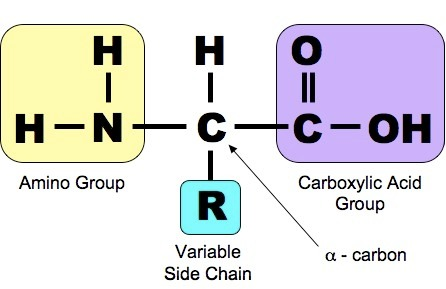
\includegraphics[width=0.55\textwidth]{amino_acid_med.jpg}

\caption{\small{The structure of an $\alpha$-amino acid in its un-ionized form. Every $\alpha$-amino acid has a carbon atom, called an $\alpha$-carbon, C$_\alpha$; bonded to a carboxylic acid, --COOH, group; an amino, --NH$_2$, group; a hydrogen atom; and an R group that is unique for every amino acid. %Note, C$_\alpha$ is a chiral center, that is to say, this carbon atom is attached to four different groups. Chirality refers to a molecule that has optical activity, so amino acids are optically active molecules. The only exception is glycine, the simplest amino acid, in which R = H.
}}

\label{fig:AminoAcid}
\end{minipage} 
\end{figure}

In addition to these 20 $\alpha$-amino acids there are many less common ones. Some are residues modified after a protein has been synthesized, others are amino acids present in living organisms but not as constituents of proteins, and two are special cases found in just a few proteins. Actually, in spite of the great number of amino acids discovered in nature (more then 700), the analyses of a vast number of proteins from almost every conceivable source have shown that all proteins are composed of 20 standard amino acids 
\cite{wu2013amino}.

To indicate the composition and sequence of amino acids polymerized in proteins, two standard codes can be used to refer briefly to amino acids:
\begin{itemize}
\item[$\triangleright$] A transparent three-letter code, where the letters are taken from the first three letters of the name of the corresponding amino acid and are pronounced as written.
\item[$\triangleright$]  A one-letter code, devised by Margaret Oakley Dayhoff (considered by many to be the founder of the field of bioinformatics), is quite less intuitive reflecting an attempt to reduce the size of the data files used to describe amino acid sequences, in an era of punch-card computing
\cite{nelson2008lehninger}. 
\end{itemize}
%the common amino acids of proteins have been assigned three letter abbreviations and one-letter symbols, which are used as shorthand to indicate the composition and sequence of amino acids polymerized in proteins. 
%A transparent three-letter code, where the letters are taken from the first three letters of the name of the corresponding amino acid and are pronounced as written. A one-letter code, devised by Margaret Oakley Dayhoff (considered by many to be the founder of the field of bioinformatics), is quite less intuitive reflecting an attempt to reduce the size of the data files used to describe amino acid sequences, in an era of punch-card computing
%\cite{nelson2008lehninger}. 
Moreover, two conventions to identify the carbons in an amino acid are used, one that makes use of numeric label and the other that uses Greek characters.
\begin{itemize}
\item[$\triangleright$] For the amino acids such as most of the other organic molecules, carbon atoms are simply numbered from one end, giving highest priority (C-1) to the carbon with the substituent containing the atom of highest atomic number.
\item[$\triangleright$] The additional carbons in an R group are commonly designated as $\beta$, $\gamma$, $\delta$ and so forth, proceeding out from the  $\alpha$ carbon.
\end{itemize} 
Within the first convention, the carboxyl carbon of an amino acid would be C-1 and the  $\alpha$ carbon would be C-2, that might be a bit confusing. In some cases, such as amino acids with heterocyclic R groups, the Greek lettering system is ambiguous and the numbering convention is therefore used \cite{nelson2008lehninger}.

\begin{figure}[h]
\centering
\begin{minipage}[t]{0.75\textwidth}
\centering
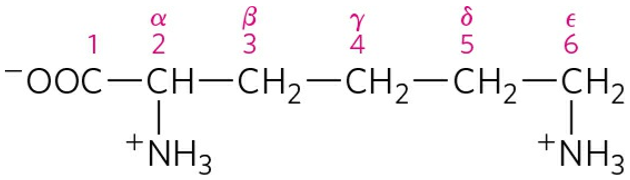
\includegraphics[width=0.65\textwidth]{Lys-cox-v2.PNG}

\caption{\small{Lysine with carbon atoms labeled by their positions.
    \textit{Source:} D. L. Nelson and M. M. Cox, ``\textit{Lehninger Principles of Biochemistry}'' (4th edition, 2008) 
    \cite{nelson2008lehninger}.}
}

\label{fig:Lysine}
\end{minipage} 
\end{figure}

It is important to note that the amino acids are dipolar ions. Indeed the amino and carboxylic acid groups of amino acids ionize readily. 
%The pK values of the carboxylic acid groups lie in a small range around 2.2, while the pK values of the $\alpha$-amino groups are near 9.4. 
At physiological pH values ($\sim$7.4), both groups are ionized, and this zwitterion\footnote{Formerly called also dipolar ion, a zwitterion is a molecule which has positively and negatively charges localized in, at least, two different functional group. The charges on the functional groups balance each other out, and the molecule as a whole is electrically neutral.} is the common form of the amino acid in solution. 
For this reason, free amino acids, like other ionic compounds, are more soluble in polar solvents than in nonpolar solvents. 

Actually, also the ionic properties of the side chains influence the physical and chemical properties of amino acids. In addition to the amino and carboxyl groups that characterize all amino acids, some amino acids have side chains with acid--base groups. The protonation or deprotonation of these functional groups determine whether the side chain has an ionic charge. Consequently, the side chains can participate in chemical reactions as acids and bases, and their ionization states determine other aspects of molecular behavior, including water solubility and the ability to interact electrostatically with other charged or polar groups
\cite{voet2016fundamentals}.

\begin{figure}[h]
\centering
\begin{minipage}[h]{\textwidth}
\centering
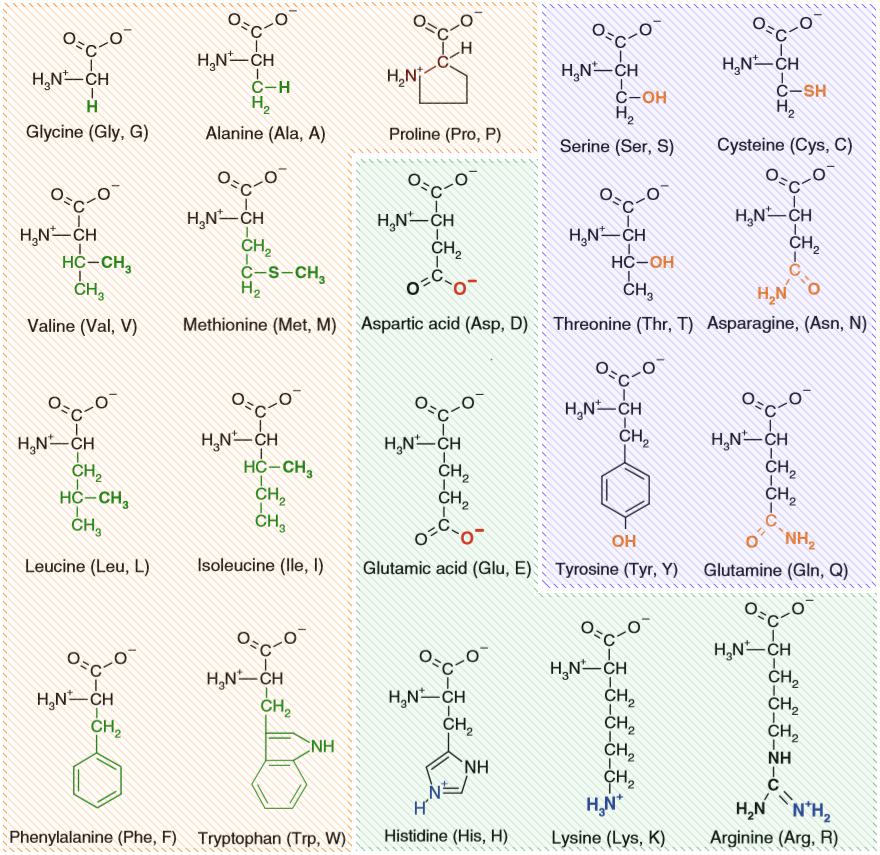
\includegraphics[width=0.9\textwidth]{std_amino_acids-buxbaum_pH7.png}

\caption{\small{The 20 standard amino acids of proteins. The structural formulas show the state of ionization that predominate at physiological pH ($\sim$7.4). The boxes divide the amino acids in three classes (\textbf{orange box}: nonpolar -- \textbf{blue box}: polar-uncharged -- \textbf{green box}: charged). Inside of each box, the functional group of the amino acids are marked: red for acidic groups, blue for the basic ones, orange for the polar-uncharged groups and green for the hydrophobic.
    \textit{Source:} E. Buxbaum, ``\textit{Fundamentals of Protein Structure and Function}'' (2007) 
    \cite{buxbaum2007fundamentals}.}
}

\label{fig:StdAminoAcids}
\end{minipage} 
\end{figure}

Indeed, knowledge of the chemical properties of the standard amino acids is central to an understanding of biochemistry. Important factors are charge, hydrophilicity or hydrophobicity, size and functional groups. These properties of the amino acids are important for protein structure and protein-protein interactions. For example: the water-soluble proteins tend to have their hydrophobic residues buried in the middle of the protein, whereas hydrophilic side chains are exposed to the aqueous solvent. Moreover, proteins that have to bind to positively charged molecules have surfaces rich with negatively charged amino acids like glutamate and aspartate, while proteins binding to negatively charged molecules have surfaces rich with positively charged chains like lysine and arginine.

Hence, this topic can be simplified by grouping the amino acids into distinct classes based on the properties of their R groups\footnote{Few amino acids are difficult to characterize and do not fit perfectly in any specific group, particularly: glycine, histidine, and cysteine. Their assignments to particular groupings are the result of considered judgments rather than absolutes
\cite{nelson2008lehninger}.}. The most useful way to classify the 20 standard amino acids is by the polarities of their side chains at biological pH, strongly related with the tendency of an amino acid to interact with water. The polarity of the R groups determine the tendency to interact with water and varies widely, from nonpolar and hydrophobic (water-insoluble) to highly polar and hydrophilic (water-soluble).

According to the most common classification scheme, there are three major types of amino acids (shown in Fig. \ref{fig:StdAminoAcids}), namely: %(1) those with nonpolar R groups (shaded orange), (2) those with uncharged polar R groups (shaded blue) and (3) those with charged polar R groups (shaded green).
\begin{enumerate}
\item \textbf{Nonpolar R Groups (}\textit{nine amino acids}\textbf{) --} %Nine amino acids.
The R groups in this class of amino acids are nonpolar and hydrophobic. Their side chains, with a variety of shapes and sizes, tend to cluster together within proteins, stabilizing protein structure by means of hydrophobic interactions.
%Phenylalanine and tryptophan contain aromatic side groups, which are characterized by bulk as well as nonpolarity.

\item \textbf{Polar-uncharged R Groups (}\textit{six amino acids}\textbf{) --} % Six amino acids.
The R groups of these amino acids are more soluble in water, or more hydrophilic, than those of the nonpolar amino acids, because they contain functional groups that form hydrogen bonds with water.%\footnote{In Particular,  Cysteine is readily oxidized to form a covalently linked dimeric amino acid called cystine, in which two cysteine molecules or residues are joined by a disulfide bond. The disulfide-linked residues are strongly hydrophobic (nonpolar). Disulfide bonds play a special role in the structures of many proteins by forming covalent links between parts of a protein molecule or between two different polypeptide chains.}
%Cysteine is unique among the 20 amino acids in that it has a thiol group that can form a disulfide bond with another cysteine through the oxidation of the two thiol groups

\item \textbf{Charged R Groups (}\textit{five amino acids}\textbf{) --} % Five amino acids.
The most hydrophilic R groups are those that are either positively or negatively charged. 
The amino acids in which the R groups have significant positive charge at pH 7.0 are lysine, arginine and histidine, while the negative ones are aspartic acid and glutamic acid (in their ionized state, they are often referred to as aspartate and glutamate). It is important to note that histidine is the only standard amino acid that, at physiological pH ranges, has a ionizable side chain near to neutrality. Consequently, both the concentration of the neutral and charged are not negligible for such pH values. In fact, the protonation-deprotonation of histidine side chains is a feature of numerous enzymatic reaction mechanisms.
\end{enumerate}

%METTERE QUALCOSA SULLA CHIRALITA'?
%Finally, an important characteristic of all the common amino acids except glycine (the simplest amino acid, in which R consists of a single H atom) is that the  $\alpha$-carbon atom is a chiral center, because it is bonded to four different groups. Due to the tetrahedral arrangement of the bonding orbitals around the C$_\alpha$, the four different groups can occupy two unique spatial arrangements, and thus for each amino acids can exist in only two configurations, named enantiomers\footnote{Since they are nonsuperimposable mirror images of each other (Fig. 3--3), the two forms represent a class of stereoisomers called enantiomers
%\cite{nelson2008lehninger}}.
%
%Note, C$_\alpha$ is a chiral center, that is to say, this carbon atom is attached to four different groups. Chirality refers to a molecule that has optical activity, so amino acids are optically active molecules. The only exception is glycine, the simplest amino acid, in which R = H.
%\\
%For all the common amino acids except glycine (the simplest amino acid, in which R consists of a single H atom), the  $\alpha$ carbon is bonded to four different groups: a carboxyl group, an amino group, an R group, and a H atom (Fig. \ref{fig:AminoAcid}; in glycine, the R group is another hydrogen atom). The  $\alpha$-carbon atom is thus a chiral center (p. 17). Because of the tetrahedral arrangement of the bonding orbitals around the  $\alpha$-carbon atom, the four different groups can occupy two unique spatial arrangements, and thus amino acids have two possible stereoisomers. Since they are nonsuperimposable mirror images of each other (Fig. 3--3), the two forms represent a class of stereoisomers called enantiomers
%\cite{nelson2008lehninger}
Finally,  it is important to note that the properties of a biomolecule that are determinant to its function are not only its covalent bonds and its functional groups, but also its stereochemistry. Indeed, the interactions between biomolecules are invariably stereospecific, requiring specific stereochemistry in the interacting molecules. The stereochemistry of a molecule is the set of its physical and biological properties that arise from the specific three-dimensional (3-D) configuration of its constituent atoms\footnote{In general, the term stereochemistry may even refer to the sub-field of chemistry, also known as 3-D chemistry, which studies the relative spatial arrangement and their manipulation of atoms that form the structure of a molecule.}.
Molecules with the same molecular formula and sequence of bonded atoms, but different configuration of their atoms are called isomers. If two isomers differ only in the spatial orientation of those atoms that cannot be rapidly interconverted by rotation about single bonds are stereoisomers. 
In fact, the main property of stereoisomers is that they cannot be interconverted without temporarily breaking one or more covalent bonds. This means that different configurations of the atoms of a specific molecule can represent different stereoisomers only if the structure of the molecule exhibits one of the following features:
\begin{enumerate}
\item Double covalent bonds in which surroundings the freedom of rotation is rather small or non-existent.
\item Chiral centers: they are those atoms of the molecule that are bounded with four different chemical species arranged in a specific orientation. 
\end{enumerate}

Hence, when two molecules differ in the arrangement of their chemical species with respect, in the first case, to the nonrotating double bond or, in the second case, to a chiral center, they are stereoisomers. They are named respectively, geometrical isomers and chiral isomers. 
In each case, two stereoisomers are well-defined compounds that can be separated from one another, and each has its own unique chemical properties. A binding site (on an enzyme, for example) that is complementary to one of these molecules would not be complementary to the other, which explains why the two compounds have distinct biological roles despite their similar chemical composition.

In the next section a short introduction to the polymerization of amino acids in peptides, polypetides and proteins is outlined.

\section{Peptide bonds and polipeptide chains}\label{sec:peptitde}
Standard amino acids can join together through a specific covalent bond to form a polymeric chain such as proteins, this type of binding is named: \textit{peptide bond}. This type of covalent bond is formed by a condensation reaction between the carboxyl group of one amino acid and the amino group of another. In this reaction a molecule of water is released as a product and the bonded amino acids that have lost the elements of water are named \textit{residue} (Fig. \ref{fig:PeptideFormation}). The two residues at both ends of a polymeric chain are distinct for the other residues.
Indeed, one of these conserves its amino group and, consequently, it is named amino-terminal (or N-terminal) residue. The other, that conserves its carboxyl group, is called carboxyl-terminal (C-terminal) residue. 
%The residue at one end of the polymer with a free amino group is named amino-terminal (or N-terminal) residue, the residue at the other end of the chain, which has a free carboxyl group, is the carboxyl-terminal (C-terminal) residue.

%Amino acids are the structural units (monomers) that make up proteins. 
%They join together to form short polymer chains called peptides or longer chains called either polypeptides or proteins. These polymers are linear and unbranched, with each amino acid within the chain attached to two neighboring amino acids.

\begin{figure}[h]
\centering
\begin{minipage}[t]{\textwidth}
\centering
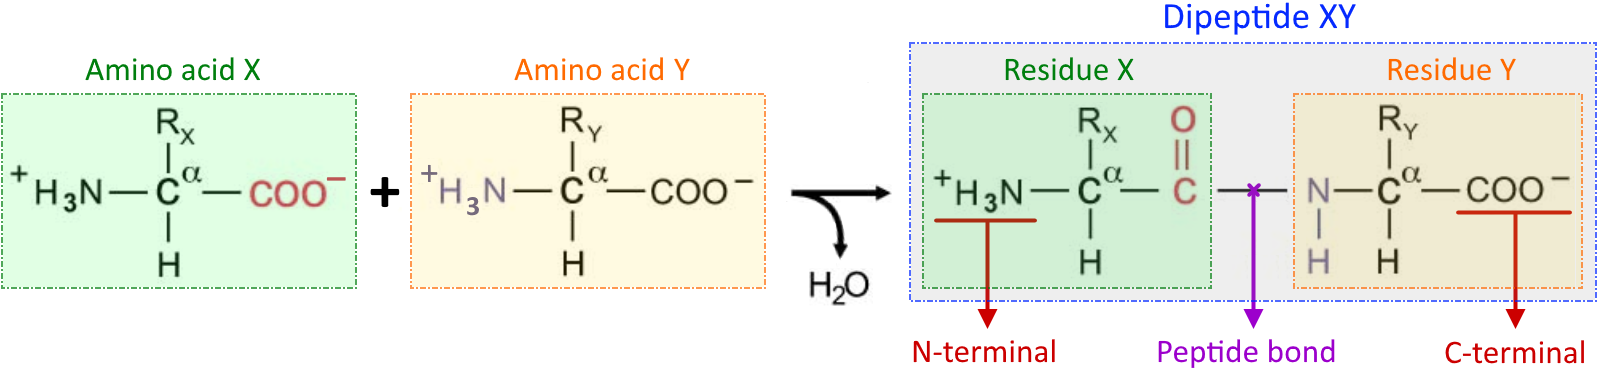
\includegraphics[width=\textwidth]{PeptideFormation-v3.PNG}

\caption{\small{General scheme of the formation of a dipeptide XY from two amino acids X and Y. The amino acids are connected through the peptide bond formed by the condensation of the carboxyl group of one amino acid with the amino group of another, producing the dipeptide. 
    \textit{Source:} T. E. Creighton, ``\textit{The Biophysical Chemistry of Nucleic Acids \& Proteins}'' (2010) 
    \cite{creighton2010biophysical}.}
}


\label{fig:PeptideFormation}
\end{minipage} 
\end{figure}

Depending on the length of the polymer chain formed by the amino acid residues, the polymer can be named in different ways to emphasize the distinct properties that the polymer has as a consequence of the number of its constituents
\cite{creighton2010biophysical}.
Precisely:
\begin{itemize}
\item[$\triangleright$] A \textbf{peptide} is a shortpolymer of a few amino acid residues with a defined sequence\footnote{Actually, the name of a peptide can change according to the number of its residues, for instance: peptide with two residues is also named \textit{dipeptide}, while a peptide with three residues is a \textit{tripeptide}.}; it usually has properties that are close to those expected from just its constituent amino acids.
\item[$\triangleright$] A \textbf{polypeptide} is a longer chain, with more amino acid residues and a defined sequence; it is usually assumed to remain unfolded and to have no special chemical or physical properties. 
\item[$\triangleright$] A \textbf{polyamino acid} is a sequence of varying lengths produced by nonspecific random polymerization of one or a few amino acids.
\item[$\triangleright$] A \textbf{protein} is a polypeptide chain with a defined length and an amino acid sequence that adopts a specific folded conformation and has special physical and chemical properties.
\end{itemize}

\begin{figure}[h]
\centering
\begin{minipage}[t]{0.85\textwidth}
\centering
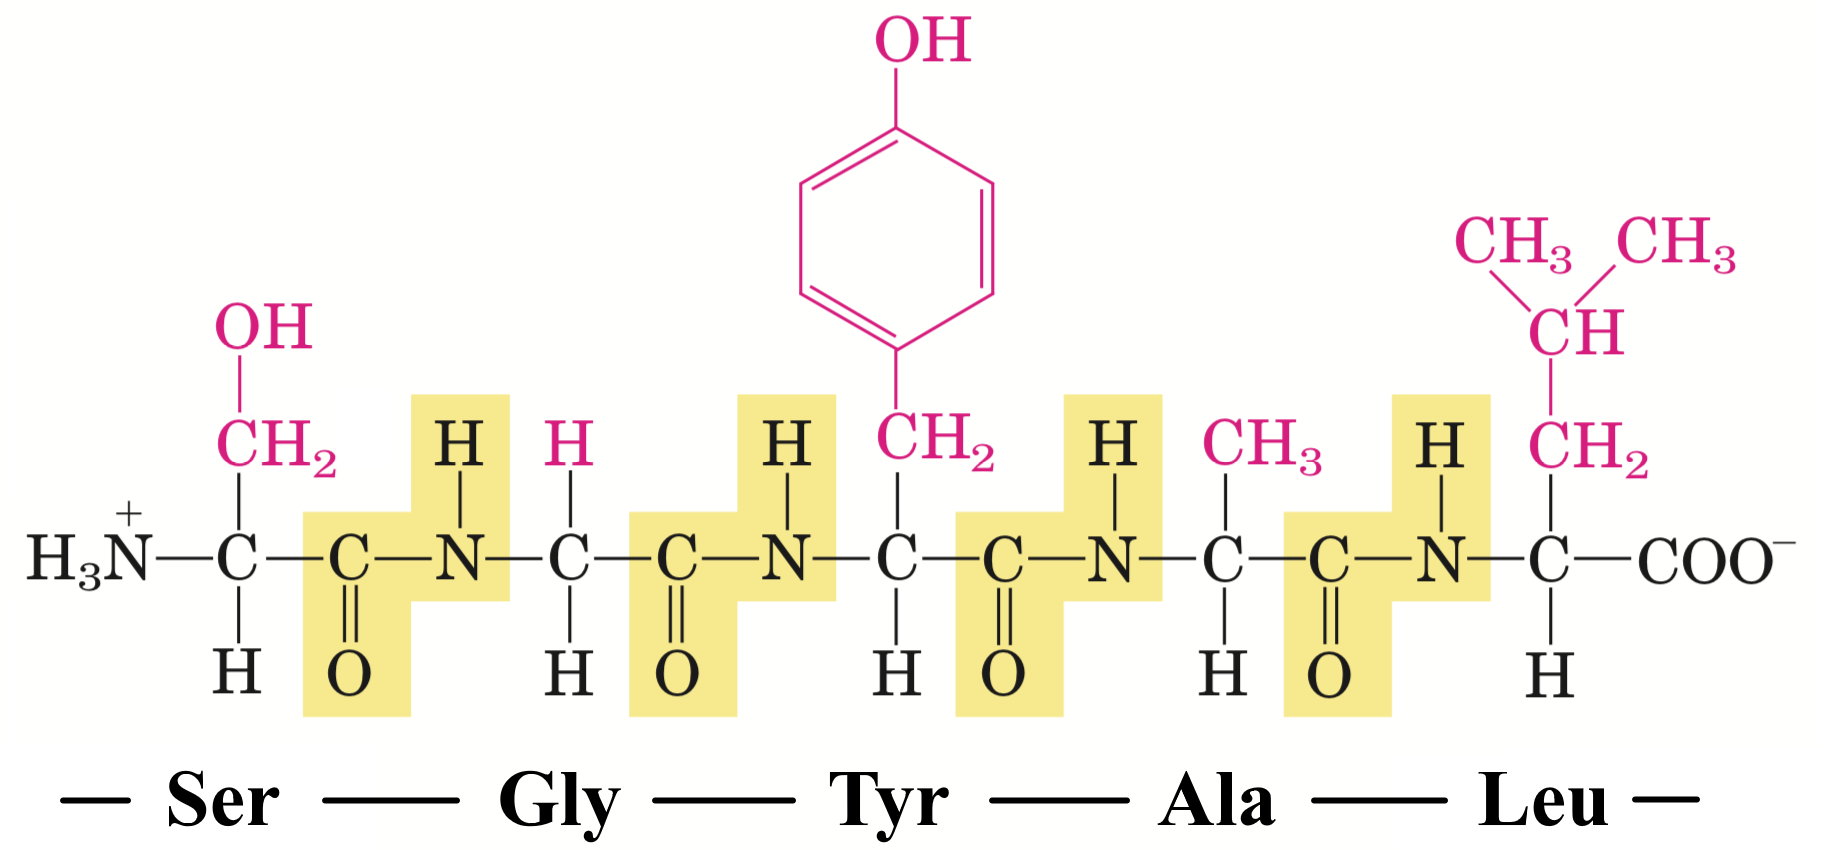
\includegraphics[width=0.68\textwidth]{Polypeptide-v3.png}

\caption{\small{Example of a peptide chain -- the serylglycyltyrosylalanylleucine. Peptide bonds are shaded in yellow; R groups are in red.
    \textit{Source:} D. L. Nelson and M. M. Cox, ``\textit{Lehninger Principles of Biochemistry}'' (4th edition, 2008) 
    \cite{nelson2008lehninger}.}
}

\label{fig:PentaPeptide}
\end{minipage} 
\end{figure}

The residues in peptides and polipeptides are named by dropping the suffix, usually -ine, in the name of the amino acid and replacing it by -yl. Peptide chains are described by starting from the N-terminal residue;  and proceeding to the C-terminal one. The amino acid at the C-terminus is given the name of its parent amino acid without alterations. Obviously, such names for polypeptide chains of more than a few residues are extremely complicated. Hence, the pentapeptide in Fig. \ref{fig:PentaPeptide} can also be written as Ser-Gly-Tyr-Ala-Leu using the three-letter abbreviations, or SGYAL using the one-letter code.

At this point it is important to focus on the fact that, actually, all molecules have structures that extend to three dimensions. In addition, since molecules are not rigid entities, these structures are non static. On the contrary, they can vibrate and incur also in conformational modifications of their shape as a consequence of the thermal motions. Hence, molecules do not posses a single fixed structure, but several possible configurations that, in some cases, which may result in a \textbf{well-defined average structure}.
In fact, polymers generally have an intrinsic tendency to be very flexible, when no specific structure is sufficiently more stable than all the others to predominate. Nevertheless, many biological macromolecules, especially proteins and nucleic acids, tend to adopt few stable conformations that produce a well-defined average structure, known as native conformation
\cite{nelson2008lehninger}. This ability of polypeptide chains to get a well-defined 3-D configuration is crucially because their biological functionality is strongly connected to their specific 3-D structure. In fact, distinct proteins adopt diverse 3-D structures and, as a consequence, they can perform different functions. 

In this way, with 20 different choices available for each amino acid residue in a polypeptide chain, it is easy to understand that a huge number of different proteins with different structures are possible. Indeed, for a protein of $n$ residues, there are $20^n$ different sequences. Hence, for a relatively small protein of 100 residues, there are $20^{100} \approx 10^{133}$ possible unique polypeptide chains of this length -- an extraordinary huge number, far greater than the roughly estimated number of atoms in the universe ($10^{80}$). Naturally, the evolution of biological systems has produced only a tiny fraction of these theoretical possibilities \cite{creighton2010biophysical}. 

It is just thanks to this peculiarity of the proteins to adopt, generally, an average structure that enables them to carry out several specific biological activities, and also to their polymeric nature, that allow to obtain a great diversity of biomolecules built up with the same fundamental constituent, that these type of bio-polymer are of central importance for leaving organism and this explains also why there is a huge number of different proteins in cells.  

%However, not all the possible sequences have the same stability, some limitations of their composition and in their size may occur.
However, there are some \textbf{constrains on the allowed composition of protein sequences and their size}. 
Indeed, the three-dimensional structure of a polypeptide chain is due to the relative interactions between its various residues. Therefore, as a consequence of the various physico-chemical properties that the amino acid residues exhibit, some sequences may be more stable than others -- the characteristics of an individual protein depend more on its amino acid sequence than on its amino acid composition
\cite{voet2016fundamentals}. 
This leads to the fact that the 20 standard amino acids do not appear with equal frequencies in proteins. Actually, the most recurring residues in proteins are Leu, Ala, Gly, Val, Glu, and Ser, while the less frequents are Trp, Cys, Met, and His. 

With respect to the constrains in size of the protein chains, these are related to the number of interactions between the residues and the limitations of the protein biosynthesis process.
%the coding capacity and the efficiency of the protein biosynthesis.
%\item the dimensions of the cells
%\item the transcription and translation errors
%The first is a lower bound limitation. 
Indeed, to maintain a well-defined average structure, that is a key feature for a protein, the interactions between the residues that tend to stabilize the structure have to overcome the thermal agitation. However, for small chains (less than 40 residues) the interactions are often not enough and, consequently, they tend to lack a defined structure.\footnote{As reported at the beginning of this section, these chains are named peptides and not proteins.} %\footnote{It is quite important to note that, even if a sequence has more than 40 residues, this do not ensure a defined structure. However, for short chains, having a well-defined average configuration is }.
On the other hand, protein sequences cannot be indiscriminately long, as a consequence the genetic coding capacity of nucleic acids and the accuracy of the protein biosynthetic process. In fact, there is a linear correspondence between the sequence of a gene\footnote{A gene is a sequence of DNA which encodes a polypeptide sequence.} in the nucleic acid and the amino acid sequence of the protein for which it codes. Hence, the length of a protein in a cell must be short enough to be encoded in the nucleic acids of its cell \cite{nelson2008lehninger}. Moreover, the second factor limiting the size of proteins is the error frequency during protein biosynthesis. This type of error is low (about 1 ``wrong'' amino acid per 10,000 residues added), but even this low rate results in a high probability of a damaged protein if the protein is very long. Therefore, the longer the polypeptide (and the longer its corresponding mRNA), the greater the likelihood of introducing errors during its synthesis. 
%However, there are some limitation in composition size and  of the protein chains.
Practically, proteins have between 100 and 1000 residues, with an average of 355 residues. The shortest proteins contain at least 40 residues while the largest have more than 30 thousand residues\footnote{The largest known protein is the mouse titin protein with 35,213-residues -- a giant protein, greater than 1 $\mu m$ in length with more than half a million of atoms, that functions as a molecular spring which is responsible for the passive elasticity of muscles.}.

%It is simply more efficient to make many copies of a small polypeptide than one copy of a very large protein. In fact, most proteins with a molecular weight greater than 100,000 have mul- tiple subunits, identical or different
 %However, the vast majority of polypeptides  
%Multisubunit proteins contain several identical and/or nonidentical chains called subunits. Some proteins are synthesized as single polypeptides that are later cleaved into two or more chains that remain associated.

At this point, before briefly summarizing the main aspects of the protein structures, it is useful to clarify the concept of \textbf{molecular conformations}.
%Actually, just as it is explain in more details in the next section, proteins can be described in terms of levels of organization

%8.2. RANDOM-COIL POLYPEPTIDE CHAINS (RIMANE)\\
%The substantial flexibility of the polypeptide chain gives it significant conformational entropy (section \ref{sec:configurational-entropy}
%1.3) and makes the random coil the most favored conformation under many conditions. 
%\cite{creighton2010biophysical}\\

%\textbf{There Are Several Levels of Protein Structure}\\
%For large macromolecules such as proteins, the tasks of describing and understanding structure are approached at several levels of complexity, arranged in a kind of conceptual hierarchy. Four levels of protein structure are commonly defined. A description of all covalent bonds (mainly peptide bonds and disulfide bonds) linking amino acid residues in a polypeptide chain is its primary structure. The most important element of primary structure is the sequence of amino acid residues. Secondary structure refers to particularly stable arrangements of amino acid residues giving rise to recurring structural patterns. Tertiary structure describes all aspects of the three-dimensional folding of a polypeptide. When a protein has two or more polypeptide subunits, their arrangement in space is referred to as quaternary structure. Primary structure is the focus of Section 3.4; the higher levels of structure are discussed in Chapter 4.


Different conformations are nonidentical spatial arrangements of the atoms of a molecule achieved solely by rotations about single covalent bonds. %Molecules with identical covalent structures but different conformations are known as conformers.
Any conformation of a molecule %of known covalent structure 
can be specified by the rotations about its single bonds, generally measured by either the torsion angle or the dihedral angle\footnote{A dihedral angle is the angle between the two planes identified by two sets of three atoms, having two atoms in common -- four distinct atoms in all. If the four atoms are linked by consecutive covalent bonds, the dihedral angle is also called proper dihedral angle or torsion angle, otherwise the dihedral angle is known as an improper dihedral angle or improper torsion angle.}. In general, interactions between neighboring atoms shall ensure that not all bond rotations have the same free energy and are equally probable (see Fig. \ref{fig:EthaneConf}).


\begin{figure}[h]
\centering
\begin{minipage}[t]{0.85\textwidth}
\centering
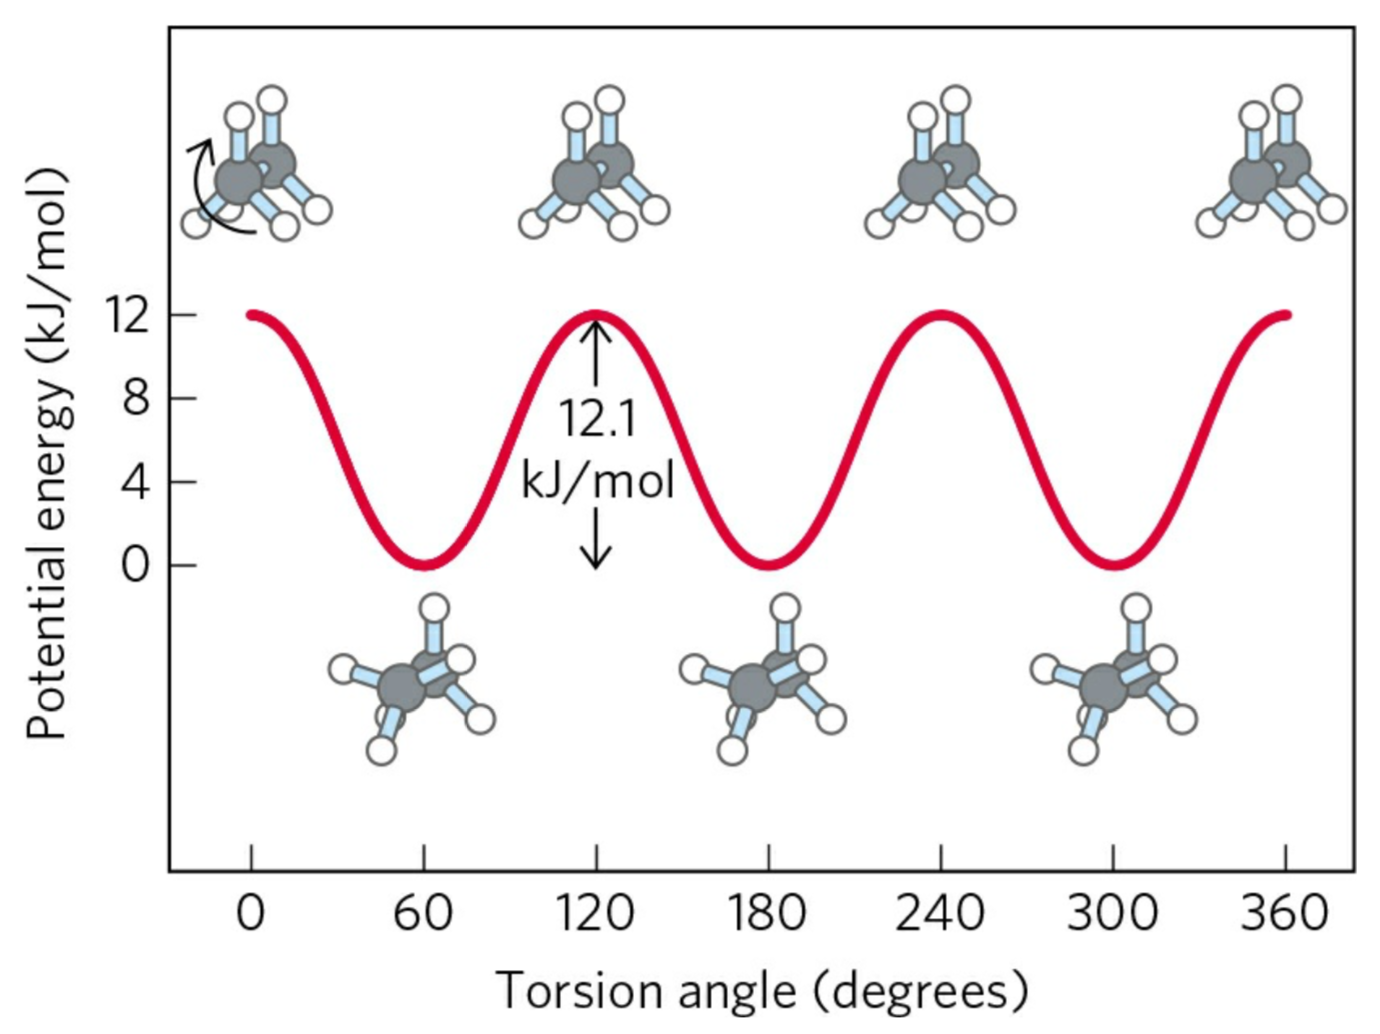
\includegraphics[width=0.6\textwidth]{conformations.png}

\caption{\small{An example of the way the potential energy of a simple molecule changes among the several conformations that the molecule assume for different values of its torsion angle. The shown molecule is ethane and it is interesting to note that in this case the energy differences, compared to the thermal energy at room temperature ($\approx 2.5 \text{kJ}/\text{mol}$), are small enough to allow rapid interconversion of the two limit forms -- millions of times per second.
    \textit{Source:} D. L. Nelson and M. M. Cox, ``\textit{Lehninger Principles of Biochemistry}'' (7th edition, 2017) 
    \cite{nelson2017lehninger}.}
}

\label{fig:EthaneConf}
\end{minipage} 
\end{figure}


%Large biological macromolecules are able to have stable 3-D structures (they native conformations), if they have sufficient stabilizing interactions between its various atoms. 

On the other hand, even though a great part of the conformation of a macromolecule seems fixed and, for this reason, it is considered a single conformation, parts of the molecule may still be flexible and able to undergo rotations about certain bonds, as a consequence of the thermal agitation. Actually, the average overall conformation can be considered as a \textbf{macro-conformation}, whereas the variations resulting from flexibility define various \textbf{micro-conformations}. The interchange of different macro-conformations requires a cooperative change of a number of bond rotations simultaneously, while micro-conformations are interconverted by changes of just one or a few bond rotations. These cooperative changes will in general happen only slowly or less frequently under physiological conditions. This relatively slow interconversion of the two macro-conformations is described as a conformational change, in which the macromolecule has been converted from one family of micro-conformations to an experimentally distinguishable family of other micro-conformations
\cite{creighton2010biophysical}.

%In the case of a protein, its conformations will depend whether on the structures and conformational properties of their residues that on the environment -- especially the relative interactions of the protein with the solvent and with itself.

The tendency to adopt a great number of conformations is an entropic factor that stabilizes the flexible state, known as the conformational entropy.
%In this picture, the conformational entropy is a measure of the ability to adopt a number of such conformations that stabilizes the flexible state. 
A single conformation will be adopted only if the interactions stabilizing that particular conformation are sufficiently strong to overcome the \textbf{conformational entropy} tending to keep the protein unfolded. The number of micro-conformations and the conformational entropy of proteins can be huge. For a protein with $n$ residues, if each residue is able to adopt an average of $k$ conformations, the total number of conformations possible will be approximately $k^N$. For example, even a short protein of 100 residues in which each residue could adopt only 2 different conformations could assume $2^{100} \approx 10^{33}$ different protein conformations. Hence, if all these conformations have similar free energies, the probability to find the protein in a specific configuration is extremely small. 

At 25$^\circ$ C, the free energy contribution of the conformational entropy for a protein in which each residue can adopt 10 conformations will be $1.36 \;\text{kcal}/\text{mol}$ per residue. Consequently, to maintain a stable conformation, the stabilizing interactions between the atoms in that conformation have to lead to a decrease of the potential energy greater than $1.36 \;\text{kcal}/\text{mol}$ per residue in order to overcome the decrease in entropy. In the absence of such stabilizing interactions, a polymer will tend to exist in many different conformations. 

It has been observed that of the many conformations that are theoretically possible in a protein containing hundreds of single bonds, one or (more commonly) a few\footnote{The need for multiple stable conformations reflects the changes that must take place in most proteins as they bind to other molecules or catalyze reactions.} conformations generally predominate under biological conditions\footnote{These predominant conformations are usually the ones that are thermodynamically the most stable, having the lowest Gibbs free energy.}. Such stable conformations can be considered macro-conformations, in contrast to the micro-conformations that are adopted only temporarily
\cite{creighton2010biophysical}.
%Proteins in any of their functional, folded conformations are called native proteins and the macro-conformations, in turn, are named as \textbf{native conformations}.
In particular, since proteins, in favorable conditions of the surrounding environment, naturally adopt such folded macro-conformations specific, these macro-configurations are usually named as \textbf{native conformations}. %, characteristic of each proteins. 

%Of the many conformations that are theoretically possible in a protein containing hundreds of single bonds, one or (more commonly) a few generally predominate under biological conditions. 



In the next section the structure of proteins are discussed in further detail.

\section{Protein structure: four levels of complexity}\label{sec:prot-structure}
For many years, the knowledge of the atomic nature of proteins was rather inaccurate and vague and the main idea was that proteins had a random structure. Between the late 20's and first 30's, several proteins had been crystallized and these findings were the evidence that even very large proteins are discrete chemical entities with \textbf{unique structures}. 
%This conclusion revolutionized thinking about proteins and their functions, but the insight it provided was incomplete. Protein structure is always malleable in sometimes surprising ways. Changes in structure can be as important to a protein's function as the structure itself. 
In 1958, with an X-ray experiment, J. Kendrew and coworkers have been able to resolve, for the first time, the structure of a protein. However, since only a few years before the clearly regular double-helix structure of DNA was discovered, when researchers saw that the resolved protein's structure was really complex, influenced by the precedent discovery, they thought it lacked of regularity. This apparently absence of regularity in the protein's structure was supported by the idea that, probably, such irregularity might be the particular feature of proteins that allows them to fulfill their diverse biological roles. Nevertheless, nowadays, with over 100 thousand protein structures known and several comparisons between them, it is clear that proteins actually exhibit a remarkable degree of \textbf{structural regularity} and the multitude of biological functions that they perform are ensured by the great number of distinct proteins, each one with its distinct structure.

%Actually most of the dynamic activities in cells and organisms are caused by proteins, and the key to understanding these phenomena is their structures. Protein structures, however, consist of many atoms, often thousands, and can be extremely complex.
Actually most of the dynamic activities in cells and organisms are caused by proteins, and the key to understand these phenomena is their structures. However, since proteins consist of many atoms, often thousands, their structures can be extremely complex. Hence, the tasks of describing and understanding such structures are approached at several levels of complexity, arranged in a kind of conceptual hierarchy. In particular, four level of protein structure are commonly identified. 

The \textbf{primary structure} is the amino acid sequence. The \textbf{secondary structure} is any regular local structure of a polypeptide chain, such as $\alpha$ helix or $\beta$ sheet. 
The \textbf{tertiary structure} is the overall shape of the folded polypeptide chain, i.e. the spatial relationship of the secondary structures to one another.
The \textbf{quaternary structure} is the structure formed by the association of several polypeptide chains, usually called subunits, which function as a single protein complex.

\begin{figure}[h]
\centering
\begin{minipage}[t]{\textwidth}
\centering
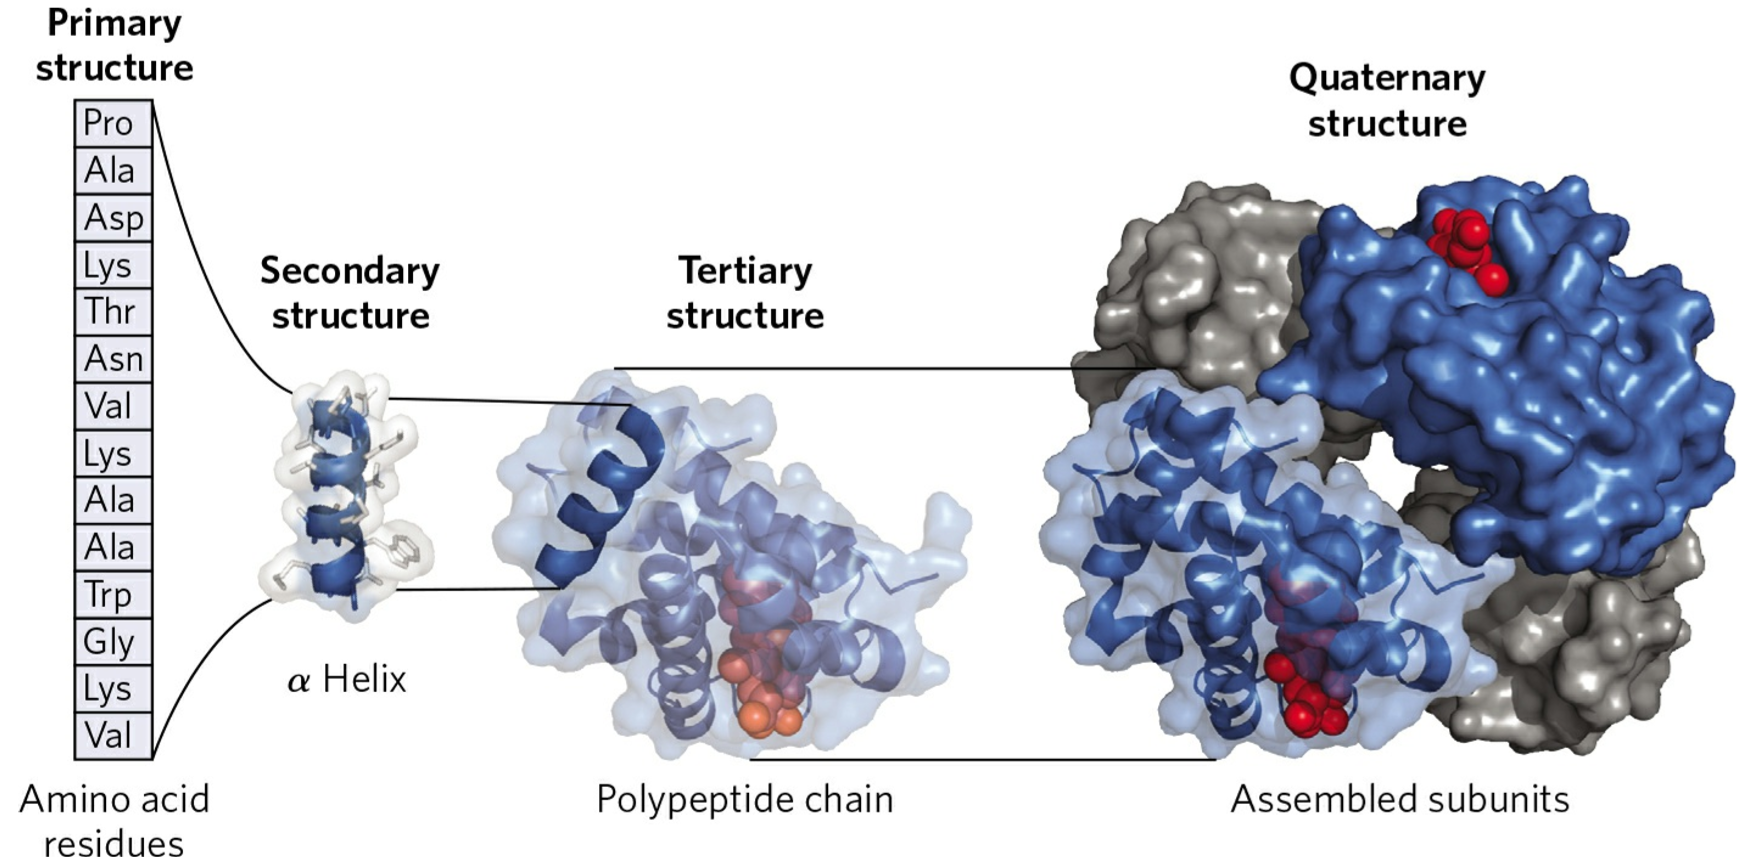
\includegraphics[width=0.95\textwidth]{Protein_structure-Cox.PNG}

\caption{\small{\textbf{Levels of structure in proteins.} The \textit{primary structure} consists of a sequence of amino acids linked together by peptide bonds. The resulting polypeptide can be coiled into units of \textit{secondary structure}, such as an $\alpha$ helix. The helix is a part of the \textit{tertiary structure} of the folded polypeptide, which is itself one of the subunits that constitute the \textit{quaternary structure} of the multisubunit protein -- in this case an hemoglobin.
    \textit{Source:} D. L. Nelson and M. M. Cox, ``\textit{Lehninger Principles of Biochemistry}'' (7th edition, 2017) 
    \cite{nelson2017lehninger}.}
}

\label{fig:ProteinStructure}
\end{minipage} 
\end{figure}

%The differences in primary structure can be especially informative. Each protein has a distinctive number and sequence of amino acid residues. The primary structure of a protein determines how it folds up into its unique three-dimensional structure, and this in turn determines the function of the protein. 

%The vast majority of the proteins, in favorable conditions of the environment, naturally fold in precise three-dimensional structures. %, characteristic of each proteins. 
%These structures are extremely different from random-coil forms of the polypeptide chain, because most of the covalent bonds in protein adopt a single dihedral angle that generally results in a folded conformation that can be considered unique and, usually, compact. This unique conformation, naturally achieved from the protein, is known as the native conformation of the protein. No changes in covalent structure need to occur when such folded conformations are adopted, except for the disulfide bonds that might be formed between Cys residues. Therefore the folded structure represents just one conformation of the many that are possible with a disordered polypeptide chain. With 20 different amino acid residues having diverse physical and chemical properties, a huge variety of protein sequences and conformations are possible. Some proteins are globular and water-soluble, others exist buried within membranes, while others adopt elongated and extended structures that serve primarily structural roles. In general, protein structure is most impressive in its diversity.

%PROTEIN STRUCTURE\\

%Actually most dynamic activities in cells and organisms are caused by proteins, and the key to understanding these phenomena is their structures. Protein structures, however, consist of many atoms, often thousands, and can be extremely complex.

%Natural proteins are also folded into precise threedimensional (3-D) structures and are very different from random-coil forms of the polypeptide chain, in that most of their covalent bonds adopt a single dihedral angle and Cys residues pair in specific disulfide bonds, rather than the spectrum possible with disordered polypeptide chains; this generally results in a folded conformation that can be considered unique. It is also very compact. No changes in covalent structure need occur when these folded conformations are adopted, except for the disulfide bonds that might be formed between Cys residues; therefore the folded structure represents just one conformation of the many that are possible with a disordered polypeptide chain. With 20 different amino acid residues having diverse physical and chemical properties, a huge variety of protein sequences and conformations are possible. Some proteins are globular and water-soluble, others exist buried within membranes, while others adopt elongated and extended structures that serve primarily structural roles (Section 8.5).
%Protein structure is most impressive in its diversity.

%Each protein is identified uniquely by its amino acid sequence, which is determined by the sequence of the gene from which the protein is produced, using the genetic code. The amino acid sequence determines all further aspects of the structure of the protein and, consequently, its functions. 
%\cite{creighton2010biophysical}.


%\textbf{The Covalent Structure of Proteins}\\
%What is it that makes one protein an enzyme, another a hormone, another a structural protein, and still another an antibody? How do they differ chemically? The most obvious distinctions are structural, and these distinctions can be approached at every level of structure defined in Figure ... 

%For large macromolecules such as proteins, the tasks of describing and understanding structure are approached at several levels of complexity, arranged in a kind of conceptual hierarchy. Four levels of protein structure are commonly defined. A description of all covalent bonds (mainly peptide bonds and disulfide bonds) linking amino acid residues in a polypeptide chain is its primary structure. The most important element of primary structure is the sequence of amino acid residues. Secondary structure refers to particularly stable arrangements of amino acid residues giving rise to recurring structural patterns. When a protein has two or more polypeptide subunits, their arrangement in space is referred to as quaternary structure.

%The differences in primary structure can be especially informative. Each protein has a distinctive number and sequence of amino acid residues. The primary structure of a protein determines how it folds up into its unique three-dimensional structure, and this in turn determines the function of the protein. 



%\textbf{THE THREE-DIMENSIONAL STRUCTURE OF PROTEINS}\\
%
%This conclusion revolutionized thinking about proteins and their functions, but the insight it provided was incomplete. Protein structure is always malleable in sometimes surprising ways. Changes in structure can be as important to a protein's function as the structure itself. 
%
%In this chapter, we examine the structure of proteins. We emphasize six themes. 
%\begin{enumerate}
%\item The three-dimensional structure of a protein is determined by its amino acid sequence. 
%\item The function of a protein depends on its structure.
%\item An isolated protein usually exists in one or a small number of stable structural forms. 
%\item The most important forces stabilizing the specific structures maintained by a given protein are noncovalent interactions. 
%\item Amid the huge number of unique protein structures, we can recognize some common structural patterns that help to organize our understanding of protein architecture.
%\item Protein structures are not static. All proteins (are in state of constant vibration and, sometimes, they) undergo changes in conformation ranging from subtle to dramatic. Parts of many proteins have no discernible structure. For some proteins or parts of proteins, a lack of definable structure is critical to their function.
%\end{enumerate}

%\textbf{The Function of a Protein Depends on Its Amino Acid Sequence} -- IMPORTANZA DELLA STRUTTURA PRIMARIA - collegamento con la funzionalità\\
%Each protein is identified uniquely by its amino acid sequence, which is determined by the sequence of the gene from which the protein is produced. Therefore, since in all cells there are thousands of the different type of proteins with their characteristic three-dimensional structure to absolve at most of the biological activities required to cell resulting in the same amount of amino acids sequences.

In this context, it is possible to figure out that there is a strong connection between the primary structure of a protein and its specific biological function. Indeed, each protein has, at the same time, a unique three-dimensional structure that determine its function and a specific sequence of amino acids that identifies the protein uniquely.
Moreover, several experiments make evident that:
\begin{itemize}
\item[$\triangleright$] Proteins with different functions actually have different amino acid sequences. 
\item[$\triangleright$] Thousands of human genetic diseases have been linked to the production of defective proteins. The defect can range from a single change in the amino acid sequence to deletion of a larger portion of the polypeptide chain. Hence, if the primary structure is altered, the function of the protein may also be changed. 
\item[$\triangleright$] Comparing proteins with similar functions among different species, they often have similar amino acid sequences\footnote{An extreme case is ubiquitin, a 76-residue protein involved in regulating the degradation of other proteins. The amino acid sequence of ubiquitin is identical in species as disparate as fruit flies and humans.}.
\end{itemize}
Thus, it is clear that usually the amino acid sequence plays a fundamental role as well as in the determination of the protein's three-dimensional structure as in its function.

%In all cells there are thousands of the different type of proteins. 
%Each protein has a unique three-dimensional structure that confers, to that protein, a unique function. Each type of protein also has a unique amino acid sequence. Hence, it seems clear that amino acid sequence have to play a fundamental role in determining the three-dimensional structure of the protein, and ultimately its function. To substantiate the important relationship between amino acid sequence and biological function. 

On the other hand, some flexibility of the primary structure is possible. Indeed, proteins that carry out an almost identical function in distantly related species can also differ greatly in overall size and amino acid sequence. For most proteins 
there are distinct regions of their structure that are more relevant than others for the determination of their biological functionality. Hence, for distinct proteins that perform almost identical function, those segments of the primary structure that correspond to regions of fundamental importance for the biological functionality are the same for all proteins, while the other segments, less important for the functionality, might vary considerably. However, the fraction of the overall sequence that is relevant varies from protein to protein, complicating the task of relating sequence to three-dimensional structure, and structure to function
\cite{nelson2008lehninger}.

%On the other hand some flexibility of the primary structure is possible. Indeed, proteins that carry out an almost identical function in distantly related species can also differ greatly in overall size and amino acid sequence. Although protein that have the amino acid sequence in some regions of the primary structure might vary considerably without affecting biological function, most proteins have parts of their structure that are fundamental to their function and thus have sequences that are conserved. This bring to light that, for a protein, there are parts of its structure that are more relevant than others for the determination of its function. However, the fraction of the overall sequence that is relevant varies from protein to protein, complicating the task of relating sequence to three-dimensional structure, and structure to function
%\cite{nelson2008lehninger}.\\

%\textbf{Amino Acid Sequences Provide Important Biochemical Information} CLASSIFICAZIONE  IN FAMIGLIE DI PROTEINE - struttura PRIMARIA\\
%Knowledge of the sequence of amino acids in a protein can offer insights into its three-dimensional structure and its function, cellular location, and evolution. 
%%Most of these insights are derived by searching for similarities with other known sequences. Thousands of sequences are known and available in databases accessible through the Internet. A comparison of a newly obtained sequence with this large bank of stored sequences often reveals relationships both surprising and enlightening. 
%Exactly how the amino acid sequence determines three-dimensional structure is not understood in detail, nor can we always predict function from sequence. However, protein families that have some shared structural or functional features can be readily identified on the basis of amino acid sequence similarities. Individual proteins are assigned to families based on the degree of similarity in amino acid sequence. Members of a family are usually identical across 25\% or more of their sequences, and proteins in these families generally share at least some structural and functional characteristics. Some families, however, are defined by identities involving only a few amino acid residues that are critical to a certain function. A number of similar substructures, or ``domains'', occur in many functionally unrelated proteins. These domains often fold into structural configurations that have an unusual degree of stability or that are specialized for a certain environment. Evolutionary relationships can also be inferred from the structural and functional similarities within protein families. Certain amino acid sequences serve as signals that determine the cellular location, chemical modification, and half-life of a protein. %Special signal sequences, usually at the amino terminus, are used to target certain proteins for export from the cell; other proteins are targeted for distribution to the nucleus, the cell surface, the cytosol, or other cellular locations. Other sequences act as attachment sites for prosthetic groups, such as sugar groups in glycoproteins and lipids in lipoproteins. Some of these signals are well characterized and are easily recognized in the sequence of a newly characterized protein. 
%\\


%\\
%Differences in primary structure can be especially informative. Each protein has a distinctive number and sequence of amino acid residues. The primary structure of a protein determines how it folds up into its unique three-dimensional structure, and this in turn determines the function of the protein.\\
%
%The relationship between the amino acid sequence of a protein and its three-dimensional structure is an intricate puzzle that is gradually yielding to techniques used in modern biochemistry. An understanding of structure, in turn, is essential to the discussion of function in succeeding chapters. We can find and understand the patterns within the biochemical labyrinth of protein structure by applying fundamental principles of chemistry and physics.
%\\
%
%One of the keys to deciphering the function of a given protein is to understand its structure. %
%
%%Like the other major biological macromolecules, the nucleic acids (Section 3-2) and the polysaccharides (Section 8-2), proteins are polymers of smaller units. But unlike many nucleic acids, proteins do not have uniform, regular structures. This is, in part, because the 20 kinds of amino acid residues from which proteins are made have widely differing chemical and physical properties (Section 4-1C). The sequence in which these amino acids are strung together can be analyzed directly, as we describe in this chapter, or indirectly, via DNA sequencing (Section 3-4). 
%In either case, amino acid sequence information provides insights into the chemical and physical properties of proteins, their relationships to other proteins, and, ultimately, their mechanisms of action in living organisms. 
%\cite{voet2016fundamentals}\\
%\\


More in general, although proteins exhibit a well-defined average structure, as shown at the end of the previous section, their native configurations are only marginally stable as a consequence of the thermal agitation. Indeed, under physiological conditions, the separation in the free energy among the folded and unfolded states is typically in the range between 20 and 65 kJ$/$mol, that is comparable with the thermal energy 2.5 kJ$/$mol. Therefore, the probability that a protein changes spontaneously its configuration is usually not negligible. 
The tendency to maintain a native conformation, is usually known as the \textbf{thermal stability of the protein}. 


%\textbf{A Protein’s Conformation Is Stabilized Largely by Weak Interactions} -- COME VIENE OTTENUTA UNA CONFORMAZIONE STABILE\\
%In the context of protein structure, the term stability can be defined as the tendency to maintain a native conformation. Native proteins are only marginally stable; the $\Delta G$ separating the folded and unfolded states in typical proteins under physiological conditions is in the range of only 20 to 65 kJ$/$mol. 
Actually, on one side, the configurational entropy, along with the hydrogen-bonding interactions of many groups in the polypeptide chain with the solvent (water), tends to maintain the unfolded state. On the other side, the chemical interactions that offset these effects and stabilize the native conformation include disulfide (covalent) bonds and weak (noncovalent) interactions. The \textbf{weak interactions} is often used to refer at: hydrogen bonds, hydrophobic effect, ionic and van der Waals interactions. 

A \textbf{disulfide bond}, also called disulfide bridge, is a covalent bond derived from the oxidation of two sulfhydryl (-SH) groups present, for example, in the cystine amino acids (see Fig. \ref{fig:ss-bond}). Even if the disulfide bridges are covalent bonds, they have a typical binding energy of an intermediate magnitude between the weak noncovalent interactions (listed  and most of the other covalent bonds -- approximately 60 kcal$/$mol. Therefore, in physiologically environment, disulfide bonds are quite reversible and play a special role in the structures of some proteins by the formation of weak covalent links between parts of a polypeptide molecule or different polypeptide chains. In particular, it is interesting to observe that, although many proteins of most organism do not have disulfide bonds, typically this is not the case for the proteins of thermophilic bacteria\footnote{Thermophilic bacteria are bacteria that thrives at relatively high temperatures, usually, between 50 and more than 80 $^\circ$C.}, where their structures are stabilized by these type of bonds. Indeed, this is presumably an adaptation to life at high temperatures. 
\begin{figure}[h]
\centering
\begin{minipage}[t]{0.8\textwidth}
\centering
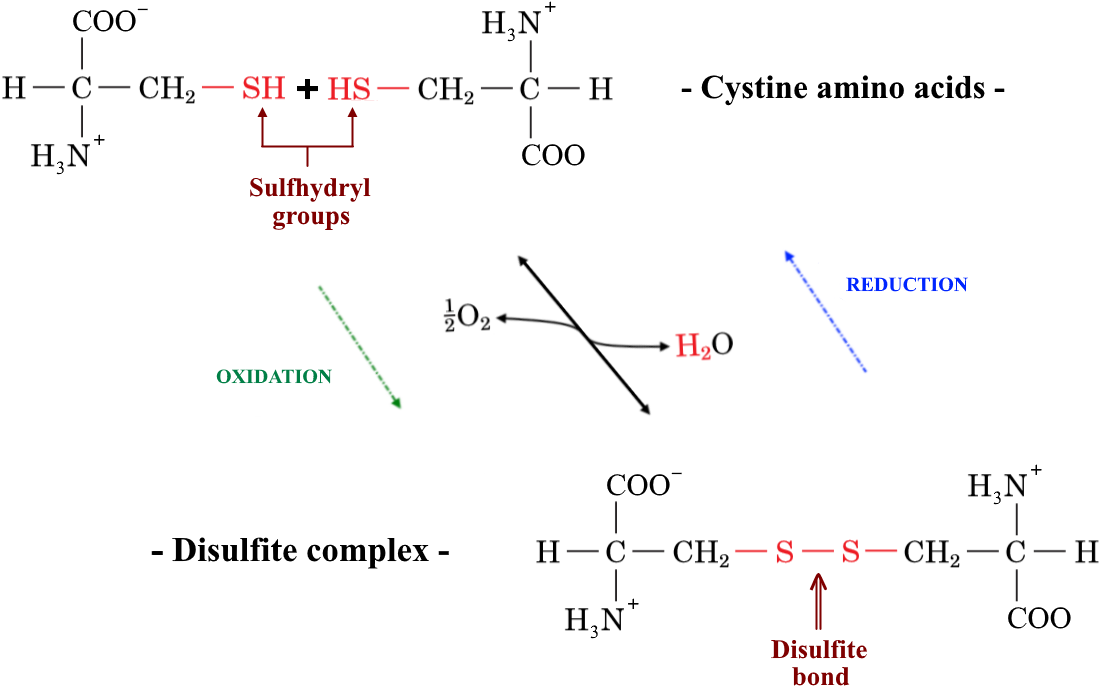
\includegraphics[width=\textwidth]{Disulfite_bond-v4.png}

\caption{\small{Reversible formation of a disulfide bond by the oxido-reduction of two molecules of cysteine. Disulfide bonds between Cys residues stabilize the structures of many proteins.}}

\label{fig:ss-bond}
\end{minipage} 
\end{figure}

On the other hand, for all proteins, \textbf{weak interactions} are especially important in the folding of polypeptide chains into their secondary and tertiary structures and the association processes of multiple polypeptides to form quaternary structures also relies on these weak interactions. However, the typical energies of the weak interactions are about 0.4 to 30 kJ$/$mol. Hence, a bond between two atoms based on such interactions might be really unstable and easy to break due to the thermal agitation.

Nevertheless, thanks to the great number of weak interactions, in favorable environment, they are able to predominate as a stabilizing force in protein structure. In general, the protein conformation with the lowest free energy (that is, the most stable conformation) is the one with the maximum number of weak interactions. However, it seems clear that increasing the temperature, these type of interactions, even if in a great number, become less important for the stabilization of protein structures until, becoming totally negligible, this leads to loss of their native conformations, unfolding into random-coil structures\footnote{For this reason, in thermophilic bacteria the disulfide bridge, having greater binding energy than weak interactions, can be useful to stabilize the structure of their proteins.}.

Moreover, the thermal stability of a protein does not depend only on the interactions between their constituent atoms, but also with the surrounding water. 
Indeed, for every hydrogen bond formed in a protein during folding, a hydrogen bond %(of similar strength) 
between the same group and water was broken. Therefore, since the energy of the first bond is practically equal as the second, the net contribution to the protein's stability for the formation of a new hydrogen bond inside a protein, from an energetic point of view, may be close to zero. 
%Ionic interactions may be either stabilizing or destabilizing. We must therefore look elsewhere to understand why a particular native conformation is favored. 
%On the hydrophobic effect

However, among the contribution of the several weak interactions that participate in the protein stabilization, the \textbf{hydrophobic effect} generally predominates, revealing the fundamental role that the water has in the thermal stability of proteins. This is a consequence of the fact that pure water contains a dense network of hydrogen-bonded H$_2$O molecules and, practically, no other molecule has the hydrogen-bonding potential of the water. Hence, the presence of non-water molecules in an aqueous solution reduces the mean number of hydrogen bonds. When water surrounds a \textbf{hydrophobic molecule}, i.e. a nonpolar molecule that is unable to interact by formation of hydrogen bonds, the hydrogen bonding interactions can occur only among the water molecules, hence to maximize the number of interactions a highly structured shell of water, or solvation layer, is spontaneously formed around the hydrophobic molecule. The water molecules in this shell, known as \textbf{hydration water},
 are more ordered than those distant to the hydrophobic molecule (bulk water). Actually, in each case the network of hydrogen-bonds is quite flickering because such bonds are continuously break and rebuild by the thermal agitation. On the other hand, the most probable configurations that the water molecules may assume driven by random motions are those that maximize the number of rebuilt hydrogen bonds. Thus, since the water in the solvation layer has less possibility to form such bonds respect to the bulk water, the number of these configurations is lower for the water in the solvation layer. That means a greater order (lower entropy) for water near to the hydrophobic molecule than those in bulk.
\begin{figure}[h]
\centering
\begin{minipage}[t]{0.8\textwidth}
\centering
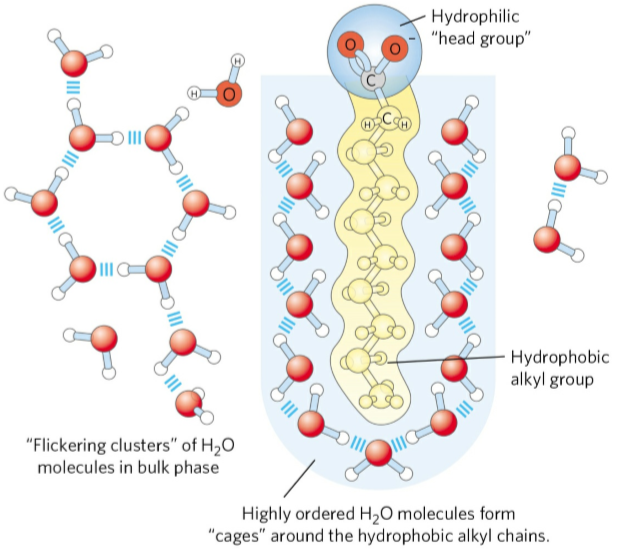
\includegraphics[width=0.7\textwidth]{hydration_shell-cox.PNG}

\caption{\small{Example of the hydrophobic ordering of the water in the solvation layer.
    \textit{Source:} D. L. Nelson and M. M. Cox, ``\textit{Lehninger Principles of Biochemistry}'' (7th edition, 2017) 
    \cite{nelson2017lehninger}.}
}

\label{fig:ss-bond}
\end{minipage} 
\end{figure}

When there are several hydrophobic molecules, if they cluster together, each group no longer exposes its entire surface to the solution, hence the extent of the overall solvation layer decreases, reducing the size of the low entropy region results in a favorable increase of the total entropy of the system. In particular, this increase in entropy is the major thermodynamic driving force for the association process of hydrophobic groups in aqueous solution. Indeed, the hydrophobic amino acid side chains tend to cluster in the inner parts of a protein, as far away as possible from water\footnote{This is the case, for instance, of the formation of oil droplet in water. The inner part of such drops is formed by hydrophobic unit.}. Furthermore, since the amino acid sequences of most proteins include a significant content of hydrophobic amino acid side chains, as a consequence of this process they form a really hydrophobic core inside the protein. In this way, most of the net change in free energy due to the aggregation of hydrophobic side chains within a protein derives from the increased entropy in the surrounding aqueous solution resulting from the burial of hydrophobic surfaces, known as \textbf{hydrophobic collapse}. 
However, more than bringing a protein to its well-defined structure by the counterbalancing of the large loss of conformational entropy, this effect constrains the polypeptide chain of a protein into a set of folded conformations that, without other interactions, would result in a random shape. 
\begin{figure}[h]
\centering
\begin{minipage}[t]{0.9\textwidth}
\centering
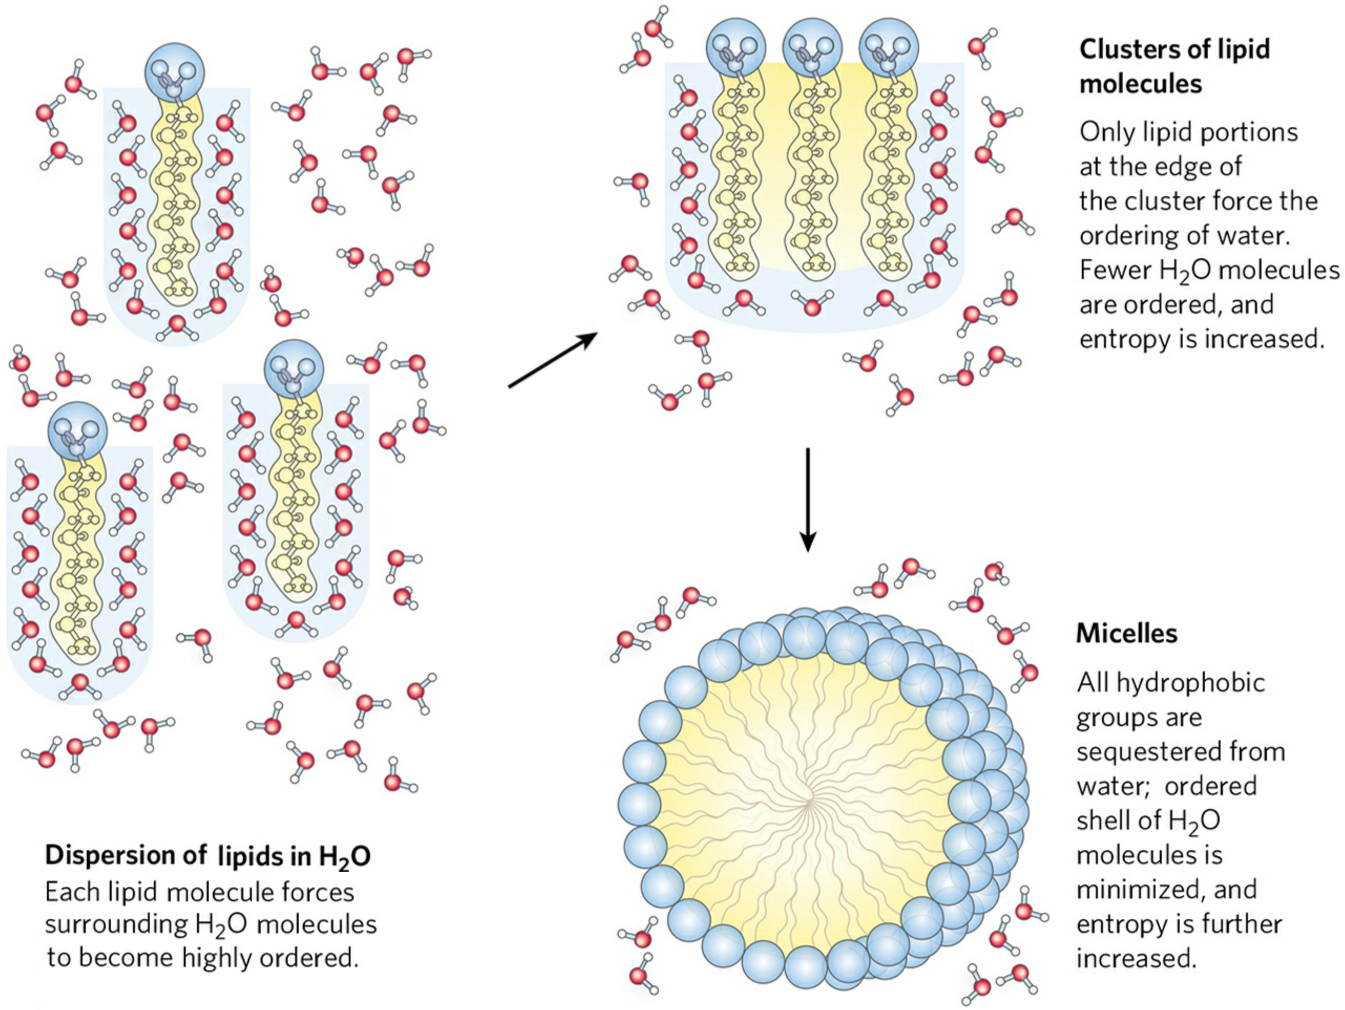
\includegraphics[width=\textwidth]{hydrophobic_effect-cox.png}

\caption{\small{Example of the hydrophobic collapse.
    \textit{Source:} D. L. Nelson and M. M. Cox, ``\textit{Lehninger Principles of Biochemistry}'' (7th edition, 2017) 
    \cite{nelson2017lehninger}.}
}
 

\label{fig:ubq}
\end{minipage} 
\end{figure}

%On the hydration water
On the other hand, under physiological conditions, the hydrophobic collapse determines also the formation of hydrogen bonds inside a protein. The number of hydrogen bonds per unit mass is generally greater for pure water than for any other liquid or solution, and there are limits to the solubility of even the most polar molecules as their presence causes a net decrease in hydrogen bonding per unit mass. In this way, a solvation layer forms to some extent even around polar molecules. Therefore, even if the energy change of the formation of an intramolecular hydrogen bond between two polar groups in a macromolecule is largely canceled by the elimination of such interactions between these polar groups and water, the release of structured water as intramolecular associations form provides an entropic driving force for the creation of hydrogen bonds within proteins which allow them to build up their characteristic three-dimensional structure. 

The hydrophobic effect is clearly crucial for protein's thermal stabilization. Nevertheless, it is also important that any polar or charged groups inside proteins have suitable partners for hydrogen bonding or ionic interactions. One hydrogen bond appears to contribute little to the stability of a native structure, but the presence of hydrogen-bonding groups without partners in the hydrophobic core of a protein can be so destabilizing that conformations containing these groups are usually thermodynamically untenable. The favorable free-energy change resulting from the combination of several such groups with partners in the surrounding solution can be greater than the free-energy difference between the folded and unfolded states. 

Moreover, hydrogen bonds between groups in a protein take place cooperatively repeating secondary structures that optimize hydrogen bonds network. In this way, hydrogen bonds often have an important role in guiding the protein-folding process. 

The interaction of oppositely charged groups that form an ion pair, also known as \textbf{salt bridge}, can provide either a stabilizing or destabilizing effect on protein structure. As in the case of hydrogen bonds, charged amino acid side chains interact with water and salts when the protein is unfolded, and the loss of those interactions must be considered when evaluating the effect of a salt bridge on the overall stability of a folded protein. However, the strength of a salt bridge increases as it moves to an environment of lower dielectric constant, $\epsilon$: from the polar aqueous solvent ($\epsilon$ near 80) to the nonpolar protein interior ($\epsilon$ near 4). Consequently, salt bridges, in particular those that are partly or entirely buried, can contribute significantly to the stabilization of the protein structure. This trend indicates that the increased occurrence of buried salt bridges in the proteins of thermophilic organisms might be useful to the thermal stability of such systems at high temperature where the stabilization induced by the hydrogen bonds becomes less significant. Ionic interactions also limit structural flexibility and confer a uniqueness to a particular protein structure not provided by the clustering of hydrophobic groups due to the hydrophobic collapse. 

In the tightly packed atomic environment of a protein the \textbf{van der Waals interactions} is further type of weak interaction that can provide a significant effect to the protein's stabilization\footnote{Van der Waals interactions are dipole-dipole interactions involving different types of dipole-dipole pair: permanent electric dipoles in groups such as carbonyls, transient dipoles derived from fluctuations of the electron cloud surrounding any atom and dipoles induced by interaction of one atom with another that has a permanent or transient dipole.}. As atoms approach each other, these dipole-dipole interactions provide an attractive intermolecular force that operates usually only over a limited intermolecular distance approximately between 0.3 to 0.6 nm. Van der Waals interactions are weak and, individually, contribute little to the overall protein's stability, but in a well-packed protein, or in the interactions between two proteins or between a protein and another molecule, the number of such interactions can be significant. 

Summarizing, most of these structural patterns already outlined for the protein folding reflect two simple main rules:
\begin{enumerate}
\item Hydrophobic residues are largely buried in the protein interior, away from water.
\item The number of hydrogen bonds and ionic interactions within the protein is maximized, reducing the number of hydrogen bonding and ionic groups that are not paired with a suitable partner.
\end{enumerate}

It is clear that the description herein presented is a simplified overview of the basic processes behind the protein folding and their thermal stability. A profound and deep study of these arguments is beyond the scope of this thesis. 
However, it is interesting to observe that, due to the high complexity of the protein's structures, the understanding of these processes is still far to be complete. The study of the protein folding and their thermal stability is an important field of research that is currently very active. One of the reasons for the scientific interest in field is that such processes are crucial in the protein structure prediction\footnote{The protein structure prediction is the inference of the three-dimensional structure of a protein from its amino acid sequence, that is the prediction of its folding and its secondary and tertiary structure from its primary structure.} that is one of the most important goals pursued by bioinformatics and theoretical chemistry, being of extremely important in medicine (for example, in drug design) and biotechnology (for example, in the design of novel enzymes). 

In the following section, a brief study focused on the protein functionality and their interactions with other molecules is presented. 
%However, a deep hunder standing folding and its secondary and tertiary structure from its primary structure
%Protein structure prediction is the inference of the three-dimensional structure of a protein from its amino acid sequence—that is, the prediction of its folding and its secondary and tertiary structure from its primary structure. Structure prediction is fundamentally different from the inverse problem of protein design. Protein structure prediction is one of the most important goals pursued by bioinformatics and theoretical chemistry; it is highly important in medicine (for example, in drug design) and biotechnology (for example, in the design of novel enzymes). 
%
%However, proteins within membranes and proteins that are intrinsically disordered or have intrinsically disordered segments follow different rules.  
%
%The example of the native 3-D structure of a small protein (ubiquitin), is shown in Fig. \ref{fig:ubq}.

%\begin{figure}[h]
%\centering
%\begin{minipage}[t]{0.8\textwidth}
%\centering
%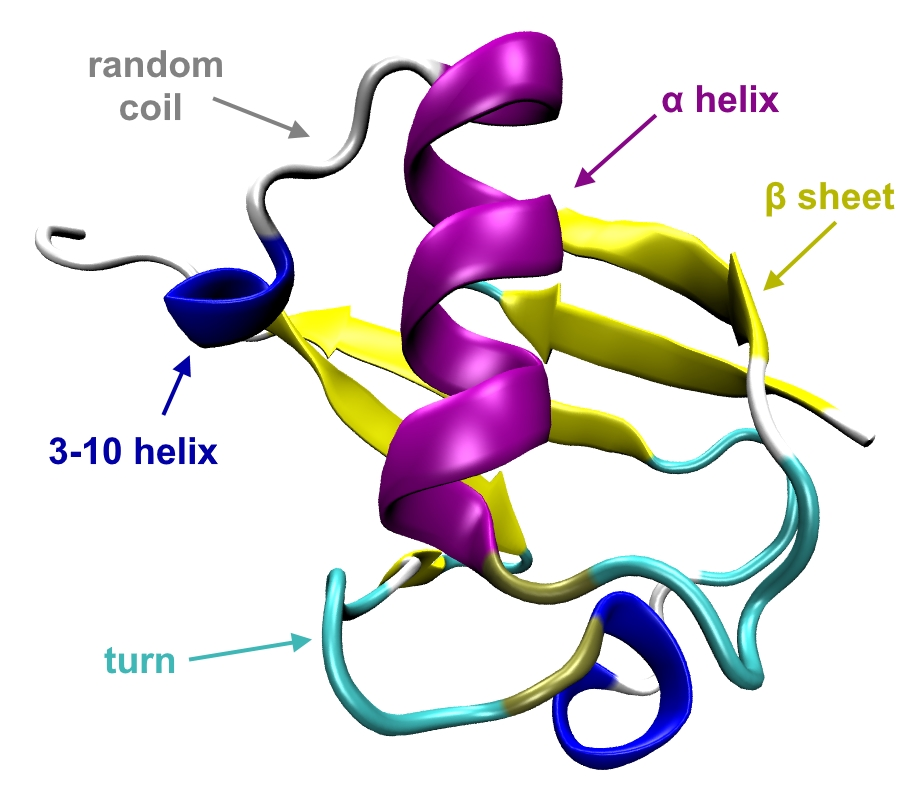
\includegraphics[width=0.75\textwidth]{ubq-label.jpg}
%
%\caption{\small{An example of a }}
%
%\label{fig:ubq}
%\end{minipage} 
%\end{figure}

%
%Nevertheless, for small molecules, since their three-dimensional (3-D) structures are relatively simple, they can be described reasonably well by two-dimensional (2-D) representations which show the bonding-connection that occur among the atoms of the molecule. Moreover, using simple drawing conventions, 2-D representations may be able to give some information on the 3-D arrangement of the atoms -- Fig. \ref{fig:ChemNot} (a).
%However, these 2-D representations cannot be used in the case of macromolecules (such as polypeptide and proteins in general) because the great complexity of their structures. For this reason, several methods to representing the 3-D structure of molecules may be used. An example of two of these methods are shown in Fig. \ref{fig:ChemNot} (b) and (c).
%
%\begin{figure}[h]
%\centering
%\begin{minipage}[t]{0.8\textwidth}
%\centering
%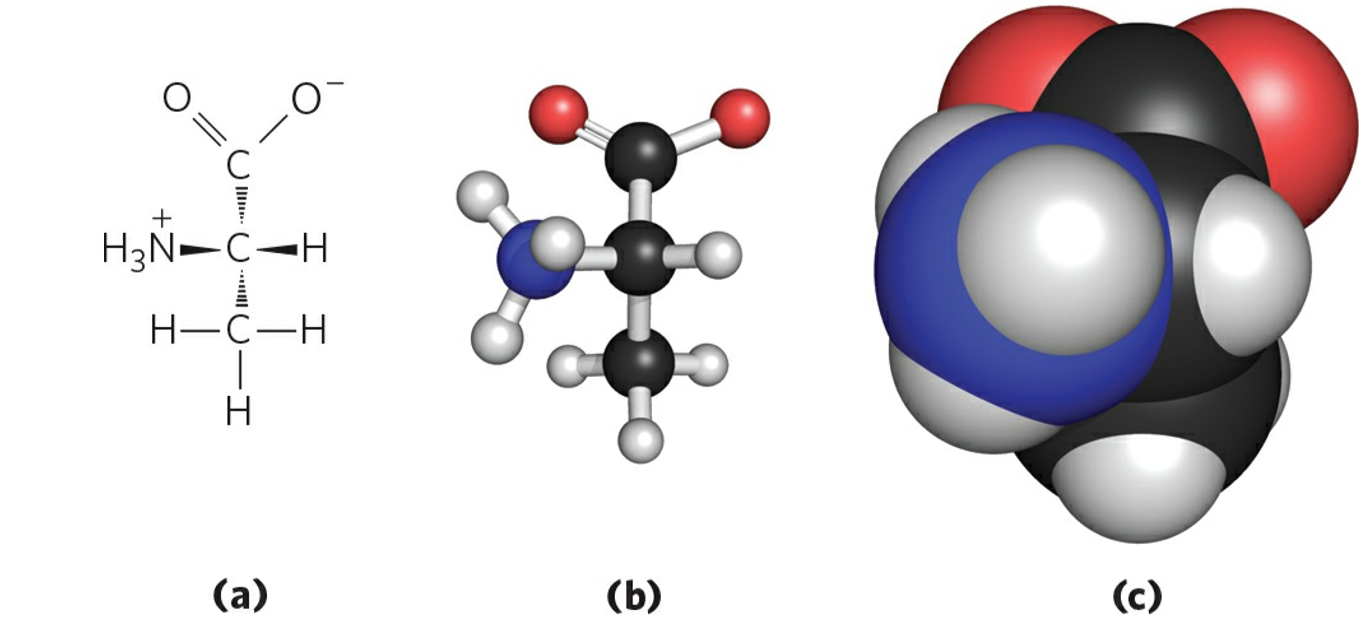
\includegraphics[width=0.85\textwidth]{ChemNotation02-cox.PNG}
%
%\caption{\small{Three models to represent a molecule. \textbf{(a)} is a 2-D representation in perspective form: solid and dashed wedge are the bonds in which the atom are out of the plane of the paper toward the reader (solid) or behind the plane of the paper (dashed). \textbf{(b)} and \textbf{(c}) are two 3-D representations. \textbf{(b)} shows bond angles and relative bond lengths. \textbf{(c)} exhibit each atom as a sphere and their edges define the space occupied by the entire molecule (the volume from which atoms of other molecules are excluded). 
%The molecule shown is an alanine
%\cite{nelson2008lehninger}.}}
%
%\label{fig:ChemNot}
%\end{minipage} 
%\end{figure}
%%At this point it is important to focus on the fact that all molecules have structures that extend to three dimensions.  Two-dimensional (2-D) chemical representations (such as \textbf{(a)} in \ref{fig:ChemNot}) usually suffice for small molecules because their three-dimensional (3-D) structures are defined reasonably well by the fixed bond lengths and bond angles of their covalent structures. 
%These representations are not sufficient for larger molecules, however, because rotations about the many covalent bonds dramatically alter the relative positions of all the atoms. 
%3-D aspects of structure are especially important for polymers such as nucleic acids and proteins, in which many bonds can rotate. In general, polymers have an intrinsic tendency to be very flexible, when no one structure, or conformation, is sufficiently more stable than all the others to predominate. However many biological macromolecules, especially the proteins and nucleic acids tend to adopt few stable conformations that produce well-defined average structures.

\section{Protein functions and protein-ligand binding}
Proteins function by interacting with other molecules. Knowing the 3-D structure of a protein is an important part of understanding protein function, and modern structural biology often includes insights into molecular interactions. However, as noted in the previous sections, proteins are not static. Actually, their interactions are affected in physiologically important ways by the protein dynamics.% sometimes subtle, sometimes striking changes in protein conformation. 

It is possible to identify two distinct type of such interactions.
\begin{enumerate}
\item In some interactions, the result is a reaction that alters the chemical configuration or composition of the interacting molecule, with the protein acting as a reaction catalyst, or enzyme.
\item In other interactions, neither the chemical configuration nor the composition of the interacting molecule is changed.
\end{enumerate}

It may seem strange that a protein's interaction with another molecule could be important if it does not alter the associated molecule. Nevertheless, transient interactions of this type are at the heart of complex physiological processes such as oxygen transport, immune function, and muscle contraction. The proteins that carry out these processes illustrate several key principles of protein function, some of which will be familiar from the study of the three-dimensional structure of the protein: 
\begin{itemize}
\item[$\triangleright$] The functions of many proteins involve the reversible binding of other molecules. A molecule bound reversibly by a protein is called a \textbf{ligand}. A ligand may be any kind of molecule, including another protein. The transient nature of protein-ligand interactions is critical to life, allowing an organism to respond rapidly and reversibly to changing environmental and metabolic circumstances. 
\item[$\triangleright$] A ligand binds at a site on the protein called the \textbf{binding site}, which is complementary to the ligand in size, shape, charge, and hydrophobic or hydrophilic character. Furthermore, the interaction is specific: the protein can discriminate among the thousands of different molecules in its environment and selectively bind only one or a few types. A given protein may have separate binding sites for several different ligands. These specific molecular interactions are crucial in maintaining the high degree of order in a living system. (This discussion excludes the binding of water, which may interact weakly and nonspecifically with many parts of a protein. In Chapter 6, we consider water as a specific ligand for many enzymes.) 
\item[$\triangleright$] Proteins are flexible. Changes in conformation may be subtle, reflecting molecular vibrations and small movements of amino acid residues throughout the protein. A protein flexing in this way is sometimes said to ``\textit{breathe}''. Changes in conformation may also be more dramatic, with major segments of the protein structure moving as much as several nanometers. Specific conformational changes are frequently essential to a protein's function. 
\item[$\triangleright$] The binding of a protein and ligand is often coupled to a conformational change in the protein that makes the binding site more complementary to the ligand, permitting tighter binding. The structural adaptation that occurs between protein and ligand is called induced fit.
\item[$\triangleright$] In a multisubunit protein, a conformational change in one subunit often affects the conformation of other subunits. 
\item[$\triangleright$] Interactions between ligands and proteins may be regulated, usually through specific interactions with one or more additional ligands. These other ligands may cause conformational changes in the protein that affect the binding of the first ligand.  
\end{itemize}

The \textbf{enzymes} represent a special case of protein function. They bind and chemically transform other molecules. The molecules acted upon by enzymes are called reaction substrates rather than ligands, and the ligand-binding site is called the catalytic site or active site. 

%As you will see, the themes in our discussion of noncatalytic functions of proteins in this chapter -- binding, specificity, and conformational change -- are continued in Chapter 6, with the added element of proteins participating in chemical transformations.

In this thesis it is studied the noncatalytic functions of proteins.

%%\section{Ligand binding process}
%The biological functions of macromolecules almost invariably depend upon their direct physical
%interaction with other molecules. All organisms and cells survive only because they interact
%effectively with their environments. Extraneous molecules must be distinguished as either useful or
%dangerous and dealt with accordingly. Organisms have sophisticated sensory organs for being aware
%of their environments. At a lower level, all cells have a variety of receptors for different molecules
%for this purpose. Virtually every small molecule in a cell was first bound specifically by the enzyme
%that produced it or by the receptor on the cell that enabled it to enter that cell. Every aspect of the
%structure, growth and replication of an organism depends upon proteins binding small molecules,
%other proteins, nucleic acids, polysaccharides or lipids. Of crucial importance is the specificity of such
%interactions. In the crowded interior of a cell, each molecule must interact only with the appropriate
%molecules and not with any of the others that are present, often in extremely high concentrations.
%The following discussion will be general but will apply primarily to proteins binding smaller ligands,
%such as their substrates for enzymatic reactions, although the catalytic events that take place after
%binding on the enzyme will be saved for Chapter 14.
%Only binding to specific sites on a protein will be considered here, and phenomena such as the
%electrostatic binding of counterions to a polyanion or polycation (Section 2.3) will not be considered
%here as ligand binding. Likewise, little attention will be given to interactions with normal components
%of the solvent, such as water molecules and co-solvents in the case of water-soluble proteins and lipids
%in the case of membrane proteins. These interactions are not fundamentally different but they do
%not occur at specific sites on the protein and are generally weak, occurring only because the solvent
%molecules are present at high concentrations
%
%12.1. GENERAL PROPERTIES OF PROTEIN-LIGAND INTERACTIONS
%Proteins usually bind only very specific ligands and can discriminate between closely related
%molecules. This specificity is usually crucial for their biological functions. Proteins are generally
%classified according to the purpose and consequences of their binding; examples are structural
%proteins, enzymes, repressors, lectins, toxins, immunoglobulins, hormones, receptors, membrane
%transport proteins and proteins of motility. The physical principles of the interactions are similar in
%all these cases. The following discussion focuses on the protein; whatever molecule it interacts with,
%even if another protein, is designated the ligand. A protein with its ligand bound is known as the holo
%form; that without the ligand is the apo form. Some examples of specific complexes are illustrated in
%Figure 12- 1.
%\cite{creighton2010biophysical}
%
%\newpage

%\section{The free-energy landscape and conformational entropy}\label{sec:configurational-entropy}
%\section{Hydration water}
\section{Thermodynamics of the binding process}\label{sec:configurational-entropy}



%The understanding of how ligands bind to proteins is of fundamental importance in biology and medicine.\footnote{The structures of protein-ligand complexes at atomic resolution make possible, for example, the design of small-molecule drugs for the treatment of disease \cite{dunn2001protein}.} Indeed, the protein-ligand interactions are crucial for the determination of the biological functions and, as a consequence, these interactions underlie almost all processes occuring in living organisms. In fact, every aspect of the structure, growth and replication of an organism depends in general on the way the proteins bind ligands (i.e. small molecules, nucleic acids, peptides, other proteins, polysaccharides or lipid) \cite{creighton2010biophysical}.

The association processes that bring to the formation of the binding between a protein and its ligand, also known as \textcolor{ForestGreen}{protein-ligand} complexation\footnote{A protein–ligand complex is a complex of a protein bound with a ligand.}, occurs when the free-energy of the whole system (protein, ligand and solvent) is lower for the complexed state, $G^\text{(c)}$, than for uncomplexed one, $G^\text{(uc)}$. Defining the difference between $G^\text{(c)}$ and $G^\text{(uc)}$ as $\Delta G$, it is possible to divide $\Delta G$ into the following two terms:
\begin{equation*}
\label{free-en}
\Delta G = G^\text{(c)} - G^\text{(uc)} = \Delta H - T \Delta S
\end{equation*}
where $\Delta H$ is the change in enthalpy due to the electrostatic interactions, while $\Delta S$ is the change in entropy due to the variation of the number of microscopic configurations for the whole system that corresponds to the new macroscopic state, namely, the solvated protein-ligand complex.
%\begin{align*}
%\label{c-uc}
%&\Delta G < 0 \quad \Longrightarrow \quad \text{\textit{the complex state is stable}} \\
%&\Delta G > 0 \quad \Longrightarrow \quad \text{\textit{the uncomplex state is stable}}
%\end{align*}

Water deeply buried in proteins is considered to be an integral part of the folded structure. Such structural water molecules make strong H bonds with polar groups of the surrounding protein and therefore are believed to tighten the protein matrix.

Studying this association processes, it is useful to identify the favorable and unfavorable contributions to the change in the free-energy of the system. Most of the unfavorable contribution is due to the loss of the three translational and three rotational degrees of freedom that lead to a considerable decrease of the entropy of the system. Generally, it is assumed that this contribution is offset by favorable enthalpy of binding and entropic contributions, such as the hydrophobic effect, changes in the protonation state and solvent or counterion release\footnote{
%The solvent entropy change arising mainly from surface burial that results in solvent release upon binding, often makes a favorable contribution to the binding entropy due to its large positive value. 
A counterion (pronounced as two words, i.e. ``counter'' + ``ion'', and sometimes written as two words) is the ion that accompanies an ionic species in order to maintain electric neutrality. In table salt (NaCl), the sodium cation is the counterion for the chlorine anion and vice versa. %For most protein-nucleic acid complexes, for example, a major contributions to the binding free energy associated with formation of the complexes is the increase in entropy due to counterion release from the nucleic acid that results from electrostatic interactions 
%\cite{mascotti1990thermodynamic}.
}. 
Nevertheless, there are other mechanisms, due to the creation or suppression of new internal degrees of freedom in the complex, that induce a change of the intrinsic entropy of the association by which a significant amount of entropy can be lost or recovered 
\cite{tidor1994contribution}. 
For this reason, it useful to divide $\Delta S$ in two contributions:
\begin{equation*}
\label{entropy-variation:total}
\Delta S = \Delta S_\text{intr} + \Delta S_\text{solv}
\end{equation*}
where $\Delta S_\text{solv}$ is the entropy change arising from accompanying modifications of interactions with the solvent, while $\Delta S_\text{intr}$ is the intrinsic change of the entropy involved in creating a dimer from two separate molecules \cite{steinberg1963entropy}. In particular, $\Delta S_\text{intr}$ represents the variation of the entropy due to the change of the number of configurations for the protein-ligand system upon the complexation (without considering the solvent) and, because of that, $\Delta S_\text{intr}$ is usually known as $\Delta S_\text{config} = S_\text{config}^\text{(c)} - S_\text{config}^\text{(uc)}$, where $S_\text{config}^\text{(c)}$ and $S_\text{config}^\text{(uc)}$ are the configuration entropy of the complexed and uncomplexed state, respectively. 

For each of these states, the configurational entropy represents a measure of the extent of the configuration space accessible to the internal degrees of freedom of the protein-ligand subsystem. In this way, the concept of configurational entropy is strongly connected to that of free-energy landscape and, as a consequece, a full characterization of the protein-ligand free-energy landscape is of fundamental importance to understand the relationship between the configurational entropy and the protein structure and the variation of these quantities upon ligand binding and conformational change. Unfortunately, the configurational entropy is known as one of the most difficult thermodynamic quantities to estimate and the characterization of the protein free-energy landscape is a difficult task due to its complexity and, in particular, to the fact that it is rugged, i.e., it comprises numerous local minima separated by low free-energy barriers \cite{chong2015dissecting}. 

In this regard, it was a keen insight to suppose that the protein configurational entropy $S_\text{config}$ may be characterized just by two terms, namely: 
\begin{equation*}
\label{entropy-variation:configurational}
\Delta S_\text{intr} \equiv \Delta S_\text{config} = \Delta S_\text{conf} + \Delta S_\text{vib}
\end{equation*}
where  $S_\text{conf}$ is the conformational components of the configurational entropy associated with the number of accessible free-energy wells \footnote{Sometimes, specially studying the protein folding phenomena, $\Delta S_\text{config}$ and  $\Delta S_\text{conf}$ might be used interchangeably even if they are not the same. This is why, in the protein folding process usually $\Delta S_\text{vib} \simeq 0$, hence $\Delta S_\text{conf} \simeq S_\text{conf}$ \cite{karplus1987configurational}.}, whereas $S_\text{vib}$ is the vibrational component that reflects the average width of the individual wells \cite{chong2015dissecting, karplus1987configurational}.%\footnote{Although attempts to dissect the relative magnitudes of different thermodynamic effects have been criticized as not formally correct, it remains helpful in understanding protein stability to estimate these individual contributions 
%\cite{doig1995side}.}.
\begin{figure}%[h]
\centering
\begin{minipage}[t]{0.8\textwidth}
\centering
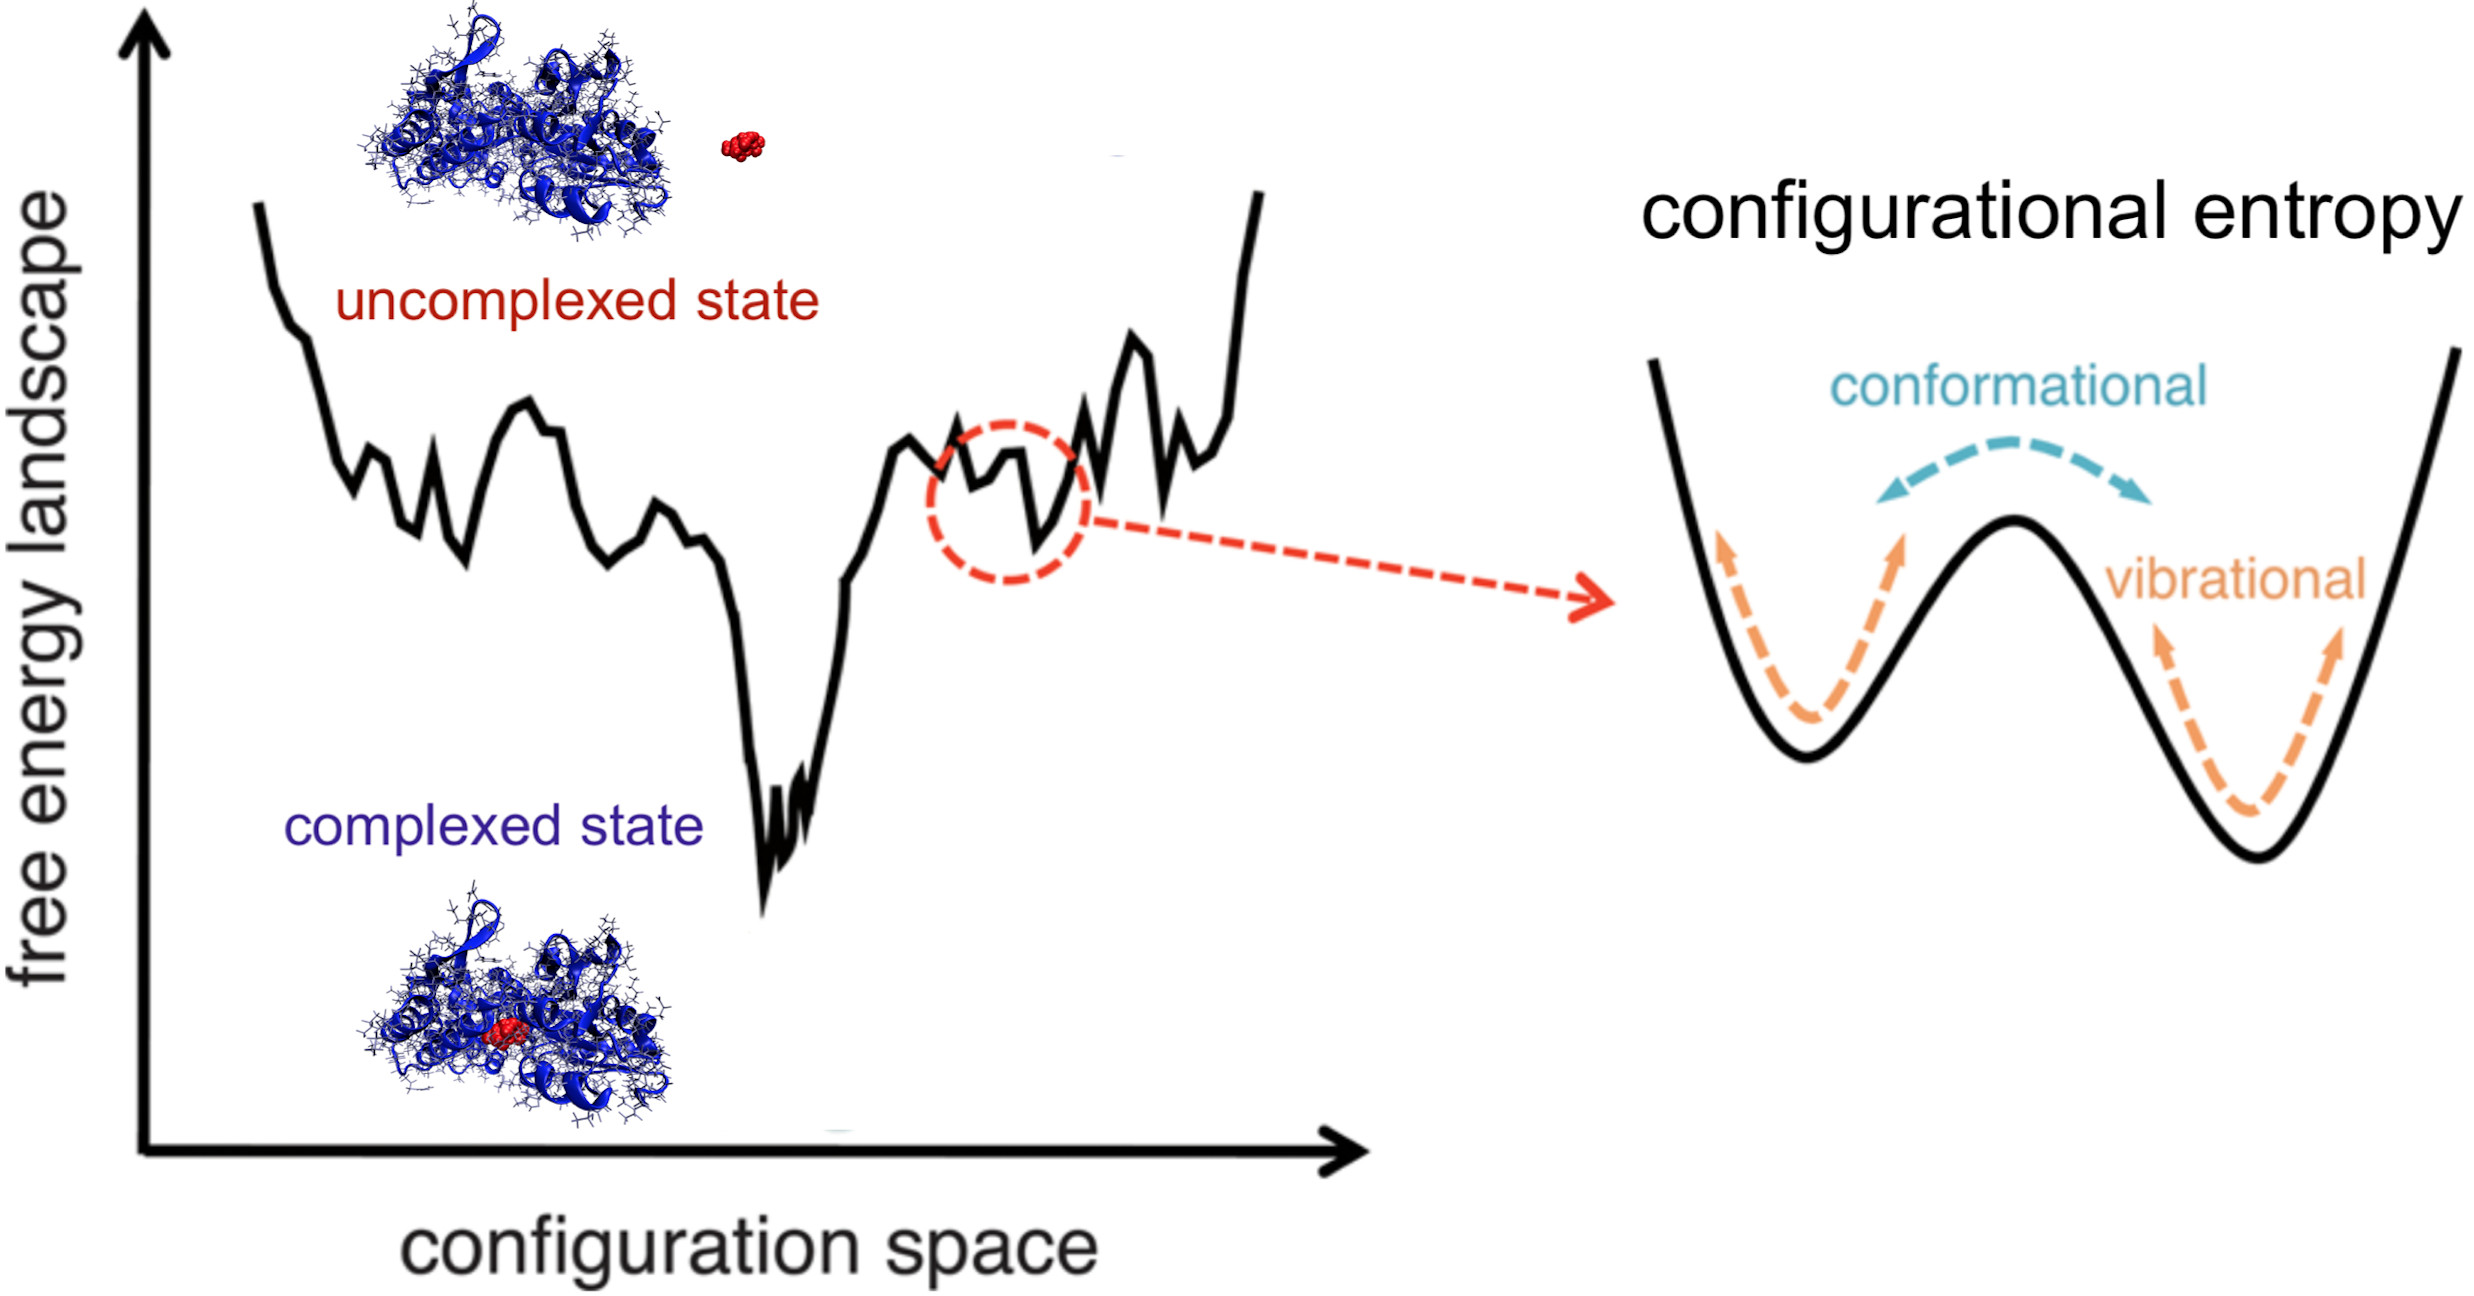
\includegraphics[width=0.8\textwidth]{free-en-landscape.jpg}

\caption{\small{Schematic representation of the free-energy landscape. Protein dynamics on the free-energy landscape can be described as a series of vibrational dynamics within individual wells and intervening conformational transitions between them \cite{chong2015dissecting}.}}

\label{fig:generation-of-microcan_state}
\end{minipage} 
\end{figure}

This subdivision of $\Delta S_\text{config}$ in two different contributions was suggested for the first time in 1981 by Karplus and Kushickt \cite{karplus1981method}. Although, in 1994, Mark and van Gunsteren criticized these types of models that attempt to decompose the free-energy into a sum of several contributions arising from different thermodynamic effects \cite{mark1994decomposition}, it has been shown that meaningful decompositions are possible and, if made carefully, they can be very useful \cite{lazaridis2002thermodynamics}.

%In 1987, Karplus et all., studying the protein denaturation, shown that, even if the $S_\text{vib}$ is typically an order of magnitude larger than $S_\text{conf}$ whether the protein is folded or not, the most important change on folding is due to $\Delta S_\text{conf}$ because the $S_\text{vib}$ is essentially the same for a protein in its native conformation and for a single conformer of the denatured polypeptide chain (i.e. $\Delta S_\text{vib} \simeq 0$ upon denaturation). 
%However, they noticed that the large magnitude of $S_\text{vib}$ raises the possibility that it may have to be considered explicitly in some cases. This is most likely when apparently small perturbations are made on the protein and a quantitative estimate of the entropy change is required. One such case is exactly the ligand binding process 
%\cite{karplus1987configurational}.

%The aim of this thesis is to evaluate of the conformational entropy change upon the complexation of a particular protein-ligand system, evaluating its conformational entropy change taking into account the effect of the formation on the binding on the hydration water.

%The aim of the thesis is to study, with molecular dynamics simulations, the association process for a specific protein and ligand system to evaluate the resulting change of conformational entropy of the system and the consequences of this change on the hydration water. Molecular Dynamics simulations are used to obtain an atomistic detail of this process. The protein and the ligand chose for the simulation are:

%\vspace{0.45cm}
%
%The objective of the thesis is to study, with molecular dynamics simulations, the protein-ligand binding in a specific case to evaluate the change of the conformational entropy upon the complexation taking into account the effect of the hydration water. Molecular Dynamics simulations are used to obtain an atomistic detail of this process.
%The protein and the ligand chose for the simulation are:
%\begin{center}
%\begin{minipage}{0.7\textwidth}
%\begin{itemize}
%\item[] \textbf{Protein:} Maltose-Binding Protein (MBP)
%\vspace{-0.2cm}
%\item[] \textbf{Ligand:} Maltose
%\end{itemize}
%\end{minipage}
%\end{center}
%MBP and Maltose have been chosen in order to compare some of the simulations' results with the measurements of inelastic neutron scattering performed on these systems by A. Paciaroni and colleges at ILL, not yet published.\footnote{MBP is a well studied model protein that plays an important role in the metabolism of Escherichia coli, e.g., in the energy-dependent translocation of maltose and maltodextrins through the cytoplasmic membrane. The ILL-EMBL Deuteration Laboratory (D-Lab) in Grenoble has developed a high-yield expression system to make available significant amounts of hydrogenated and fully deuterated MBP powder
%\cite{paciaroni2008fingerprints}.}

%On the other hand, Molecular Dynamics is one of the most widely used computer simulation techniques in material science and biophysics used to calculate the time evolution of a classical many-body system by numerically integrating Newton's equations of motion. It has two strong points, it is able to offer atomistic-level resolution and since it doesn't disrupt the kinetics of the system it allows for the calculation of transport properties and relaxation constants. However, when applied to large systems the sampling is limited by the currently available computational resources, e.g. the typical limit for a system of 100,000 atoms is the microsecond timescale. 

%For this reason, many processes of biological relevance are not accessible with the current computational power. High-probability stable and metastable states of the conformational space are separated from each other by low-probability regions, also known as energetic barriers, the transition of which is a rare event in the timescales explored by Molecular Dynamics. One example of what this practically means is that it is impossible to observe, with a single simulation (known as brute force Molecular Dynamics), the folding event of any protein other than small peptides and ultrafast folders. Hence, the biological simulated systems are usually far from ergodicity and, to improve sampling and assess thermodynamic quantities, enhanced sampling techniques are used in combination with Molecular Dynamics.\cite{kalimeri}

%
%\newpage
%
%In this regard, it was a keen insight to suppose that the protein configurational entropy ($S_\text{config}$) may be characterized just by two terms, i.e., the conformational ($S_\text{conf}$) and vibrational ($S_\text{vib}$) components.
%The conformational component is associated with the number of accessible free-energy wells, whereas the vibrational component reflects the average width of the individual wells. (Although they are often used interchangeably, we shall refer to ``conformational'' entropy as a subcategory of ``configurational'' entropy as just described.) -> questo perché nel processo di folding e unfolding $S_\text{vib} \simeq 0$ e quindi $S_\text{config} = S_\text{conf} + S_\text{vib} \simeq S_\text{conf}$
%
%Dissecting $S_\text{config}$ into $S_\text{conf}$ and $S_\text{vib}$ enables one to characterize modulations of the free-energy landscape caused by intrinsic and extrinsic factors in simple terms; furthermore, it will facilitate the discovery of molecular mechanisms underlying protein activities (in particular, those of intrinsically disordered proteins).
%
%Configurational entropy, however, is known as one of the most difficult thermodynamic quantities to estimate, and a significant amount of effort has been devoted to developing computational methods for dealing with this quantity. 
%
%Here, we propose a computational approach from a different perspective that is based on the classification of protein
%dynamics on the free-energy landscape into conformational and vibrational contributions (Figure 1). 
%
%
%\cite{karplus1987configurational}
%
%The aim of this thesis is to study 
%\newpage
%
%In this context, studying the association processes that bring to the formation of the binding between a protein and its ligand, it is possible to decompose the free energy of the association of the two molecules into a summation of favorable and unfavorable contributions. The mainly unfavorable contribution is due to the loss of the three translational and three rotational degrees of freedom that lead to a considerable decrease of the entropy of the system. Generally, it is assumed that this contribution is offset by favorable enthalpy of binding and entropic contributions, such as the hydrophobic effect, changes in the protonation state and solvent or counterion release. Nevertheless, there is another mechanism by which a significant amount of entropy can be recovered, namely, due to the creation of some new internal degrees of freedom in the complex \cite{tidor1994contribution}.
%
%Indeed, because electrostatic interactions and hydrophobic bonds are not rigid or specific and the association is an outcome of such noncovalent interactions, the associating units (i.e. the protein and the ligand) have a considerable freedom of relative motion. This freedom, corresponding to an increase in flexibility for the complex and manifested by changes in its vibrational spectrum, is able to lead to a significant positive contribution for the entropy of the association (aside from the contribution from solvent effects, such as the hydrophobic effect) \cite{steinberg1963entropy}.
%
%During the years, theoretical normal mode analyses, used to estimate this vibrational changes, have suggested that this effect is likely to be thermodynamically important and, in 2004, a first experimental determination of the vibrational changes has been achieved by Balog et al. Using inelastic neutron scattering, they showed that the vibrations of the complex soften significantly at low frequency (less then 2.5 meV) relative to the unbound protein. Deriving the resulting free-energy change from the variation in the density of states, they found that this effect contributes significantly to the binding equilibrium \cite{balog2004direct}.
%
%Anyway, there remains much to learn about the various contributions to ligand binding free energies. Indeed, whether the vibrational softening effect seen here is general for protein-ligand interactions remains to be determined. The direct access to the vibrational density of states provided by inelastic neutron scattering holds promise for the study of vibrational thermodynamic changes in many biomolecular association processes \cite{balog2004direct}. 
%
%Hence, to better understand this phenomena, in 2011 Balog et al., using computer simulations, recreated the system studied in the 2004 and reproduced the experimental results with an atomic detail normal-mode analysis to perform a characterization of the observed vibrational change.
%With these simulations they obtain several interesting results concerning the nature of the vibrational changes in the specific protein-ligand complex studied\footnote{Some of these results concern the identification of the residues most affected by ligand binding and their contribution to protein compressibility \cite{balog2011vibrational}.}. However, as they report in their paper, these results cannot be generalized to other proteins and ligands since the effect depends on the strength of the interactions involved. 
%
%Furthermore, the present analysis concentrates on the harmonic component of the dynamics.
%
%oreover, they did not explain in detail the effect that the changes in the vibrational modes of the complex have in the vibrational spectrum of the hydration water.


%\section{Experimental evidence - A brief overview of the neutron scattering results}
